\documentclass[xcolor=dvipsnames]{beamer}
\usepackage[english]{babel}
\usepackage[latin1]{inputenc}
\usepackage{times}
\usepackage[T1]{fontenc}
\usepackage{graphicx}
\usepackage[absolute, overlay]{textpos}
\usepackage{tikz}
\usepackage{multimedia}
\usepackage{soul}
\usepackage{wasysym}
\def\urltilda{\kern -.15em\lower .7ex\hbox{\~{}}\kern .04em}
\def\deg{^{\circ}}

\setlength{\TPHorizModule}{0.01\textwidth}
\setlength{\TPVertModule}{\TPHorizModule}
\definecolor{darkyellow}{rgb}{1,0.75,0}
\definecolor{black}{rgb}{0,0,0}
\definecolor{skyblue}{rgb}{0.7,0.8,1.0}
\definecolor{black}{rgb}{0,0,0}
\definecolor{darkgrey}{rgb}{0.3,0.3,0.3}
\definecolor{medgrey}{rgb}{0.5,0.5,0.5}
\definecolor{lightgrey}{rgb}{0.8,0.8,0.8}
\definecolor{lightMahogany}{rgb}{0.9,0.8,0.8}
\definecolor{darkblue}{rgb}{0,0,0.5}
\definecolor{darkgreen}{rgb}{0.1,0,0.3}
\definecolor{darkred}{rgb}{0.6,0,0}

\newcommand{\params}{\Xi}
\newcommand{\Eobsi}{E'_i}
\newcommand{\phiobsi}{\phi'_i}
\newcommand{\Etruei}{E_i}
\newcommand{\phitruei}{\phi_{i}}
\newcommand{\Eobsij}{E'_{ij}}
\newcommand{\phiobsij}{\phi'_{ij}}
\newcommand{\Etrueij}{E_{ij}}
\newcommand{\phitrueij}{\phi_{ij}}
\newcommand{\obs}{\mathrm{obs}}
\newcommand{\true}{\mathrm{true}}
\newcommand{\Like}{\mathcal{L}}
\newcommand{\ntot}{{n_\mathrm{tot}}}
\newcommand{\ntotj}{{n_{\mathrm{tot},j}}}
\newcommand{\diff}{\mathrm{d}}
\newcommand{\cblue}[1]{{\color[rgb]{0.1, 0.0, 0.6} #1}}
\newcommand{\cgreen}[1]{{\color[rgb]{0.0, 0.6, 0.1} #1}}
\newcommand{\corange}[1]{{\color[rgb]{0.9, 0.5, 0.0} #1}}
\newcommand{\cbluewhen}[2]{{\color#2[rgb]{0.1, 0.0, 0.6} #1}}
\newcommand{\cgreenwhen}[2]{{\color#2[rgb]{0.0, 0.6, 0.1} #1}}
\newcommand{\corangewhen}[2]{{\color#2[rgb]{0.9, 0.5, 0.0} #1}}

\newcommand{\manual}[1]{
  \begin{tikzpicture}[x=\textwidth, y=0.82\textheight]%, >=angle 90]
    \useasboundingbox (0, 0) rectangle (1, 1);
    #1
  \end{tikzpicture}
}

%%% Custom nodes.

\newcommand{\basenode}[4]{
  \node[outer sep=6pt, anchor=#3] (#1) at (#2){#4};
}

\newcommand{\emptynode}[2]{
  \basenode{#1}{#2}{base}{}

}

\newcommand{\minipagenode}[5]{
  \basenode{#1}{#2}{#3}{
    \begin{minipage}{#4}
      \vspace*{-12pt}
      {#5}
      \vspace*{-8pt}
  \end{minipage}}

}

\newcommand{\imagenode}[5]{
  \minipagenode{#1}{#2}{#3}{#4}{%
    \includegraphics[width=\textwidth]{#5}%
  }
}

%%% Connectors.

\newcommand{\connect}[4]{%
  \draw[<->, color=darkpurple, line width=1pt, out=#3, in=#4] (#1) to (#2);
}
\newcommand{\connectcolor}[5]{%
  \draw[<->, color=#5, line width=1pt, out=#3, in=#4] (#1) to (#2);
}
\newcommand{\hconnect}[3]{%
  \draw[<->, color=darkpurple, line width=1pt]
  (#1.east) .. controls +(right:#3) and +(left:#3) .. (#2.west);
}
\newcommand{\vconnect}[3]{%
  \draw[<->, color=darkpurple, line width=1pt]
  (#1.south) .. controls +(down:#3) and +(up:#3) .. (#2.north);
}

\newenvironment{litemize}
{\usebeamercolor[fg]{item color}%
\scriptsize\begin{list}{$\bullet$}{%
\setlength{\itemindent}{0pt}%
\setlength{\labelwidth}{10pt}%
\setlength{\leftmargin}{15pt}%
}}
{\end{list}}

\mode<presentation>
{
  \usetheme{Warsaw}
  \usecolortheme[named=Mahogany]{structure}	
  \setbeamercovered{transparent}
  \setbeamercolor*{section in toc}{bg=white, fg=Mahogany}
}

%\beamerdefaultoverlayspecification{<+->}

\AtBeginSubsection[]
{
  \begin{frame}<beamer>
    \frametitle{Outline}
  \begin{columns}[t]
	\column{0.8\textwidth}
	\tableofcontents[sections={1-3}, currentsection, currentsubsection]
  \end{columns}	
  \end{frame}
}

\setbeamertemplate{subsection in head/foot shaded}
{\textcolor{structure!70!white}{\insertsubsectionhead}}
\setbeamertemplate{subsection in head/foot}{\textcolor{white}\insertsubsectionhead}

\title[{\textcolor{white}Global Fits beyond the Standard Model with Astroparticle Data}]{\textcolor{white}{Global Fits beyond the Standard Model with Astroparticle Data}}
\author[\textcolor{medgrey}{Pat Scott -- Aug 20 -- ICIC Opening Workshop}]{Pat Scott}
\institute{\small{Department of Physics, McGill University}}
\date[Aug 20 2012]{Slides available from \color[rgb]{0.1, 0.2, 0.6} \href{http://www.physics.mcgill.ca/~patscott}{\tt http://www.physics.mcgill.ca/{\urltilda}patscott}}
\pgfdeclareimage[height=0.7cm]{university-logo}{McGill_crest}
\logo{\pgfuseimage{university-logo}}

\subject{Talks}

\begin{document}

\begin{frame}
  \titlepage
\end{frame}

\begin{frame}<beamer>
  \frametitle{Outline}
\begin{columns}[t]
  \column{0.8\textwidth}
  \tableofcontents[sections={1-3}]
\end{columns}	
\end{frame}

\section{The Problem}

\subsection{Moving beyond the Standard Model}

\begin{frame}
\frametitle{The Standard Model of particle physics}

\begin{columns}
\column{0.5\linewidth}
  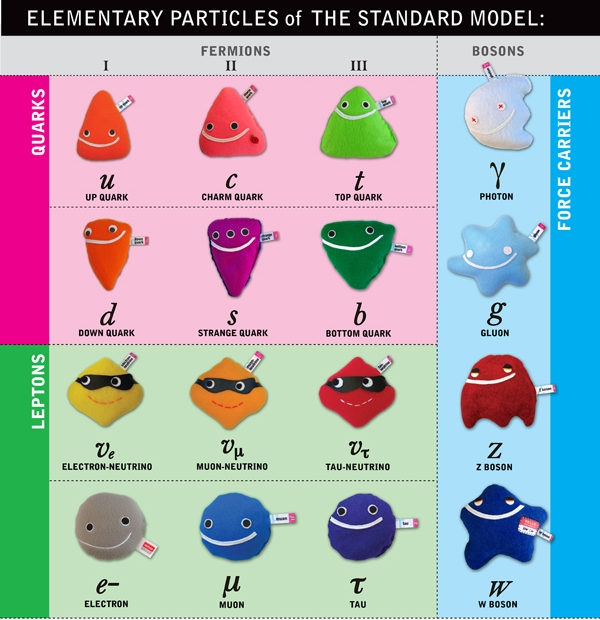
\includegraphics[width=\linewidth]{SM}
\column{0.12\linewidth}
  \centering
  \visible<2->{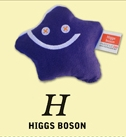
\includegraphics[width=\linewidth]{Higgs}}\vspace{5mm}
  \visible<4->{
\includegraphics[width=\linewidth]{DM}\\
  $+$friends}
\end{columns}
\vspace{5mm}

\visible<3->{\cblue{19 free parameters}: (\alert{10} masses, \alert{3} force strengths, \alert{4} quark mixing parameters, \alert{2} `vacuumy things')}

\begin{textblock}{20}(82,37)
  \visible<5->{
    \begin{tikzpicture}
      \draw[color=red,line width=0.1cm]
            (0,0) circle (0.5)
            (0,0) circle (1) 
            (1.2,0) -- (0.3,0)
            (0,1.2) -- (0,0.3)
            (-1.2,0) -- (-0.3,0)
            (0,-1.2) -- (0,-0.3);
                   	
    \end{tikzpicture}
  }
\end{textblock}


\end{frame}

\begin{frame}
\frametitle{Reasons to go beyond the Standard Model}

\begin{itemize}
\item{\cblue{Hierarchy problem} \\\hspace{3mm}\footnotesize Higgs mass receives arbitrarily large loop corrections in SM;\\\hspace{3mm}cancelled or at least truncated by new TeV-scale physics}
\item{\cblue{Vacuum stability} \\\hspace{3mm}\footnotesize With $m_h=125$\,GeV, SM Higgs mass goes negative via\\\hspace{3mm}renormalisation group running at $E<M_\mathrm{GUT}$\\\hspace{3mm}$\implies$ SM vacuum is unstable $\implies$ new particles probably stabilise it}
\item{\cblue{Dark matter} \\\hspace{3mm}\footnotesize Exists; absent in SM}
\item{\cblue{Matter-antimatter asymmetry} \\\hspace{3mm}\footnotesize More matter than antimatter; no real SM mechanism}
\item{\cblue{Neutrino masses} \\\hspace{3mm}\footnotesize Measured; absent in SM}
\end{itemize}

\end{frame}


\subsection{Beyond the SM with astroparticle probes}

\begin{frame}
  \frametitle{Dark matter -- properties \& models}
  \begin{columns}[T]
	\column{0.1\textwidth}
	
\includegraphics[width=\linewidth]{DM}
	\column{0.95\textwidth}	
	\alert<1-2>{Must be:}
        \begin{itemize}
        \footnotesize
	\item massive (gravitationally-interacting)
        \item unable to interact via the electromagnetic force (dark)
        \item non-baryonic
        \item ``cold(ish)'' (in order to allow structure formation) 
        \item stable on cosmological timescales
        \item \alert<3>{produced with the right relic abundance in the early Universe}.\\\vspace{2mm}
	\end{itemize}
        \alert<1-2>{Good options:}
        \begin{itemize}
        \footnotesize
        \item \alert<3>{Weakly Interacting Massive Particles (WIMPs)}
        \item sterile neutrinos
        \item gravitinos
        \item axions
        \item axinos
        \item hidden sector dark matter (e.g.~WIMPless dark matter)
        \end{itemize}
  \end{columns}

  \only<2-3>{
  \begin{textblock}{70}(53,63)
    \alert<2>{Bad options:}
    \begin{itemize}
      \footnotesize
      \item primordial black holes% (strong experimental constraints)
      \item MAssive Compact Halo Objects (MACHOs)%; baryonic)
      \item standard model neutrinos %(too warm; insufficient relic density)
    \end{itemize}
  \end{textblock}}

\end{frame}

\begin{frame}
\frametitle{Dark matter -- detection}

  \begin{itemize}
  \item
  {Direct detection -- nuclear collisions and recoils -- CDMS, XENON, DAMA, CRESST, CoGeNT}
  \item
  {\visible<5-9>{Direct production -- missing $E_\mathrm{T}$ or otherwise -- LHC, Tevatron}}
  \item
  \visible<7-9>{Indirect detection -- annihilations producing
  \begin{itemize}
    \footnotesize
    \item{{gamma-rays -- \emph{Fermi}, HESS, CTA}}
    \item{anti-protons -- PAMELA, AMS}
    \item{anti-deuterons -- GAPS}
    \item{{neutrinos -- IceCube}, ANTARES}
    \item{$e^+e^-$ -- PAMELA, \emph{Fermi}, ATIC, AMS}\\
    {$\rightarrow$ secondary radiation: Compton$^{-1}$,\\synchrotron, bremsstrahlung}
    \item{secondary impacts on the CMB}
  \end{itemize}}
  \item
  \visible<9>{{Dark stars -- JWST, VLT}}
  \end{itemize}
  
  \begin{textblock}{70}(40,40)
    \only<2>{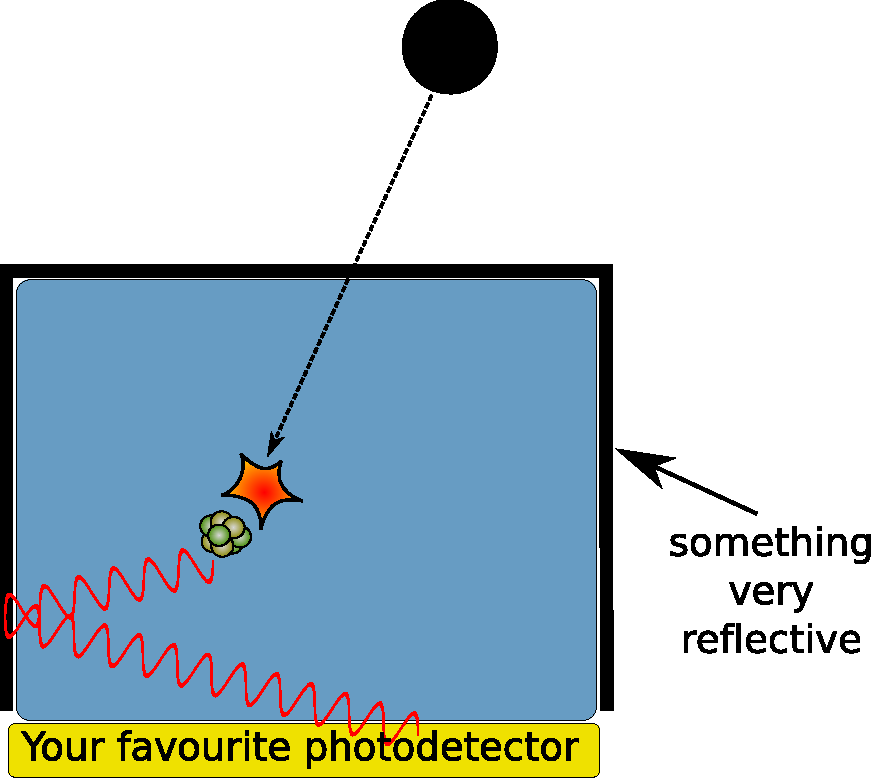
\includegraphics[width=0.6\linewidth]{SolidScintillator}}
  \end{textblock}

  \begin{textblock}{80}(25,40)
    \only<3>{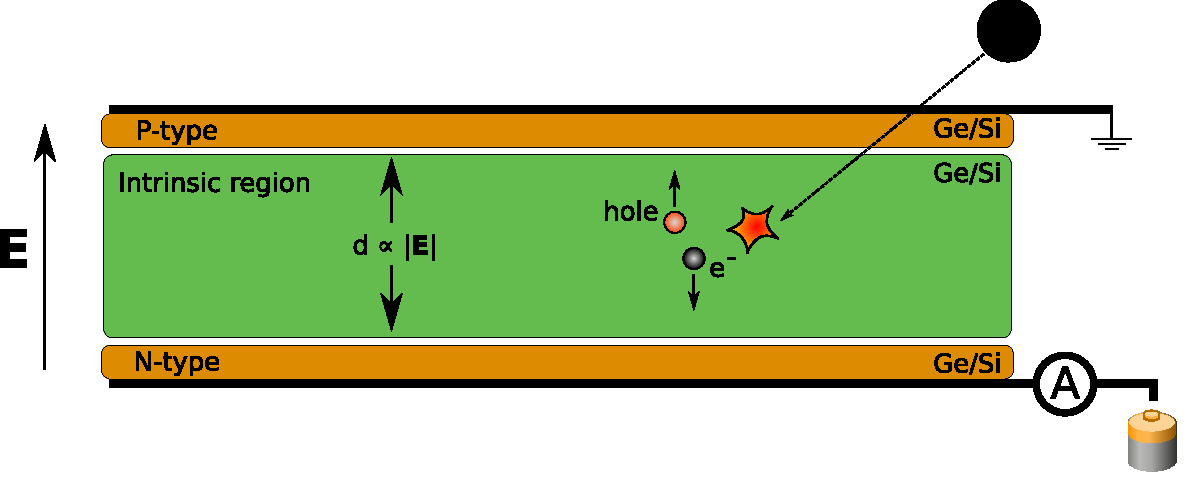
\includegraphics[width=\linewidth]{IonisationDetector}}
  \end{textblock}

  \begin{textblock}{60}(60,31)
    \only<4>{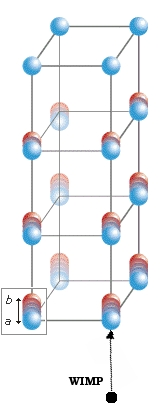
\includegraphics[width=0.35\linewidth]{Phonons}}
  \end{textblock}

  \begin{textblock}{65}(32,32)
    \only<6>{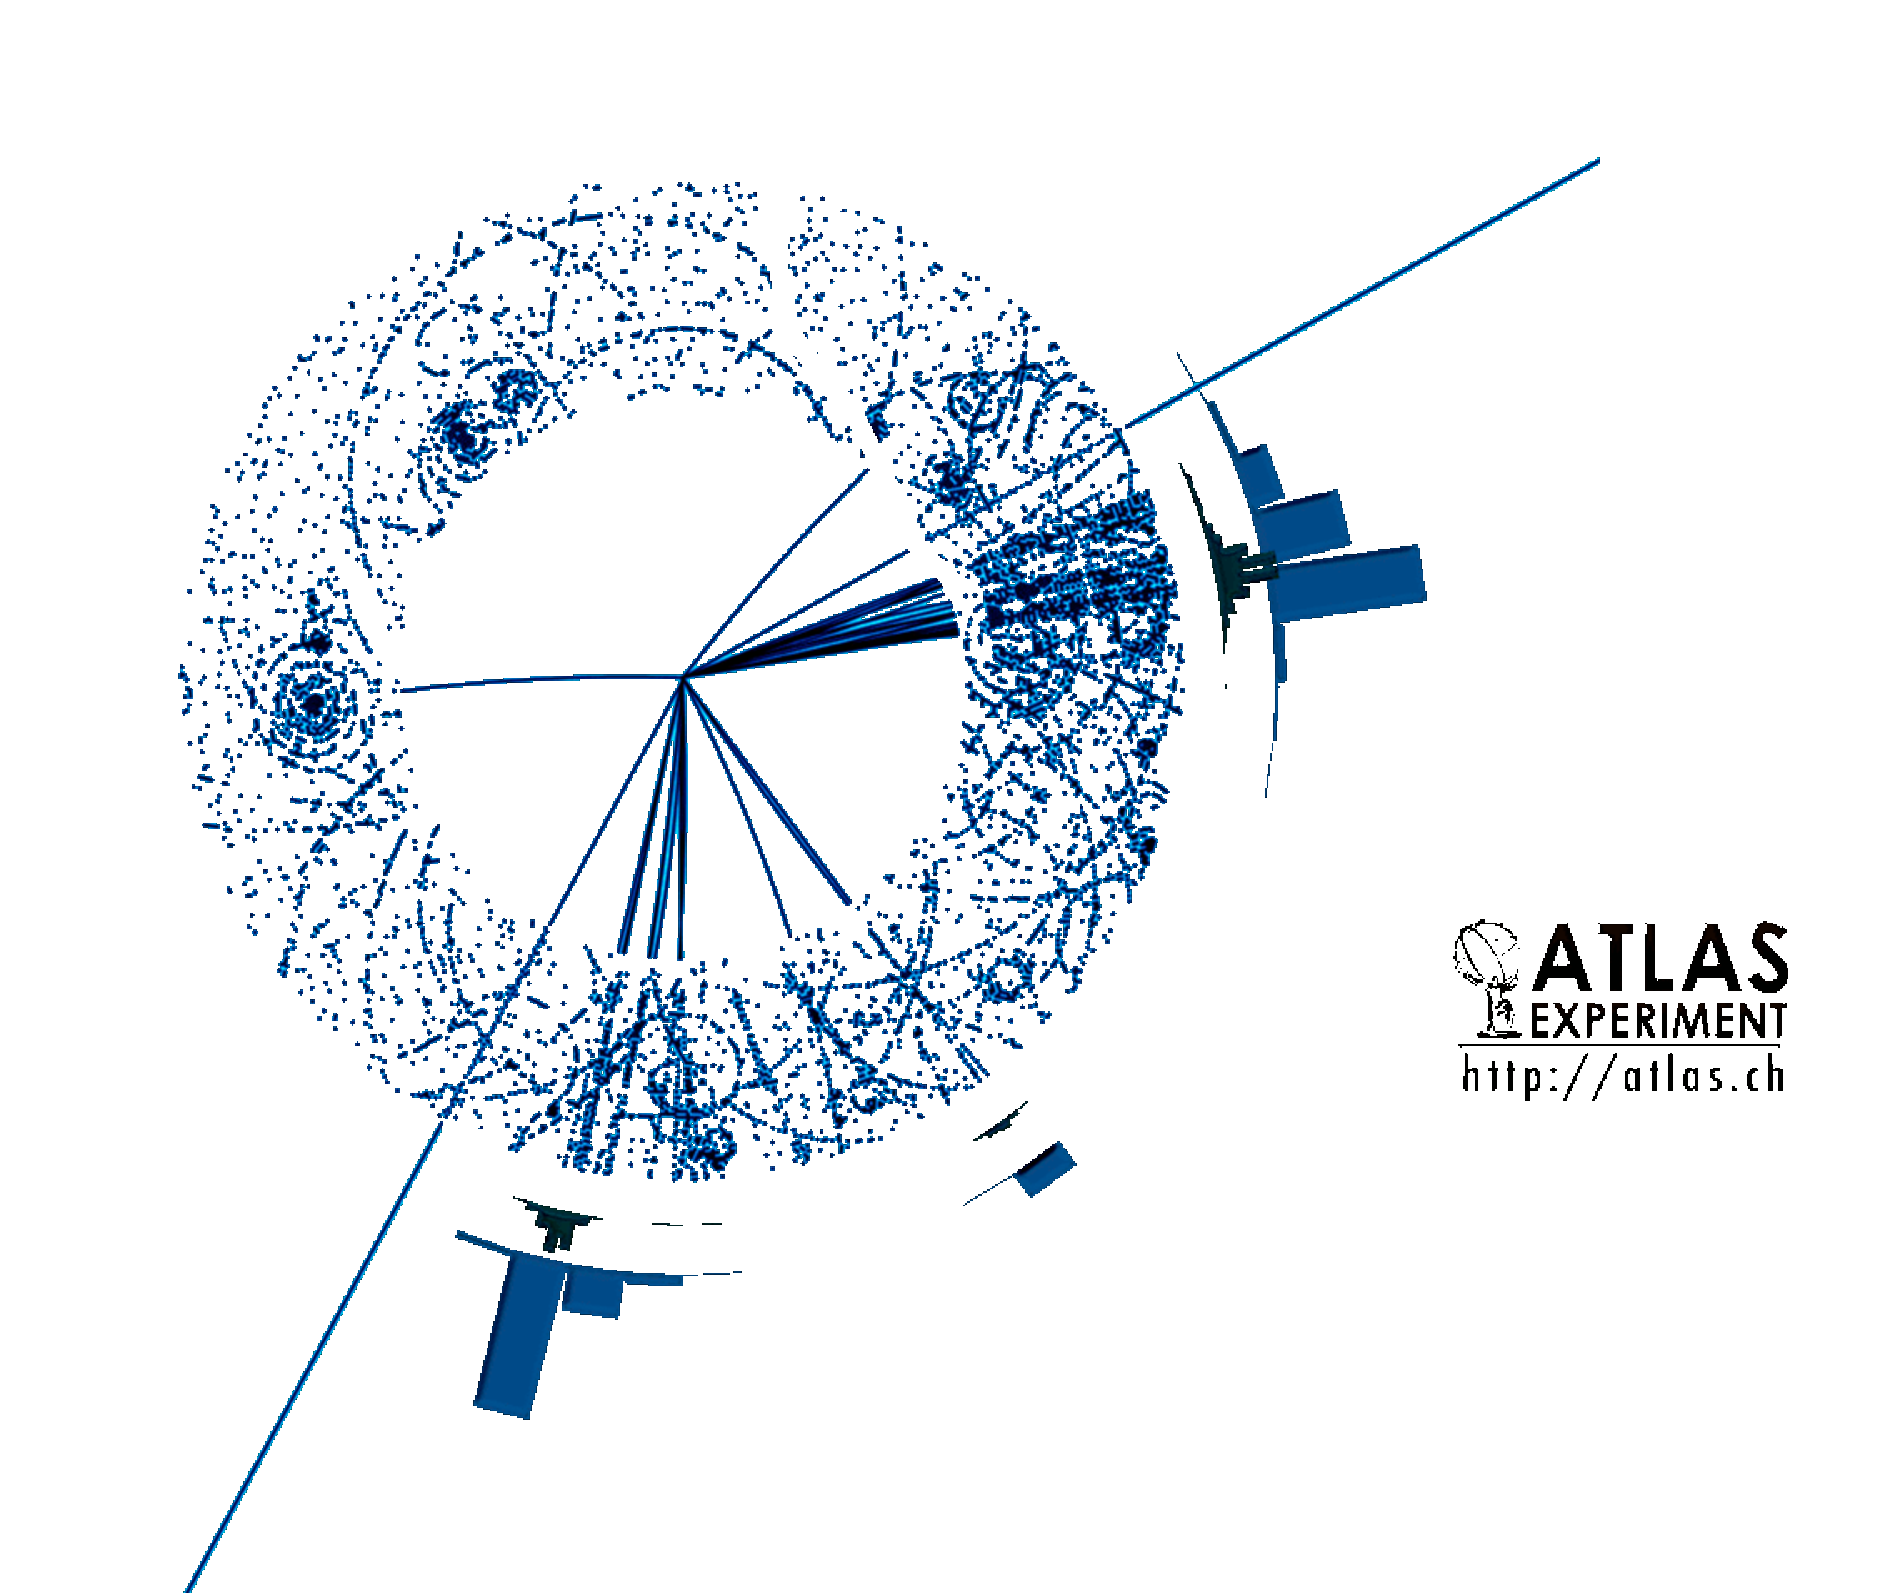
\includegraphics[width=\linewidth]{susy_sim3}}
  \end{textblock}

  \begin{textblock}{40}(75,44)
    \only<8-9>{\hspace{20mm}{\tiny Weniger (2012, \textit{JCAP})}
    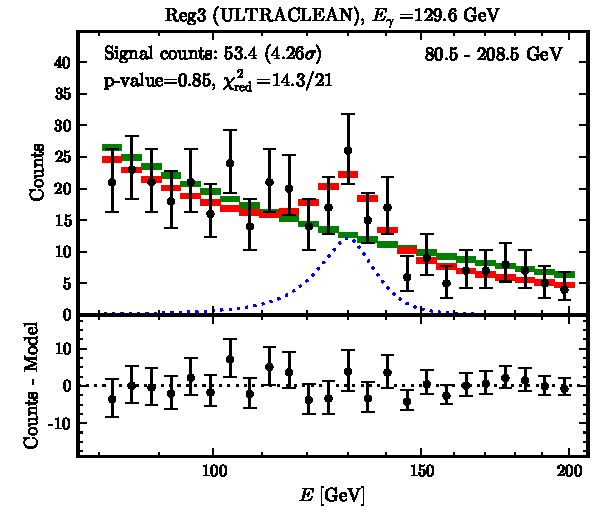
\includegraphics[width=\linewidth]{line}}
  \end{textblock}

\end{frame}


\begin{frame}
\frametitle{``The rest''}

In order of (my own completely biased opinion of) usefulness for probing BSM physics:

\begin{enumerate}
\item{\cblue{Neutrino physics (cosmological, solar, atmospheric)} \\\hspace{3mm}\footnotesize Masses, mixings, additional sterile neutrinos\\\hspace{3mm}Mass-generation models often require RH $\nu$, extra symmetry groups}
\item{\cblue{BBN} \\\hspace{3mm}\footnotesize Extra particles can change elemental yields (decays, resonances, etc)}
\item{\cblue{Baryogenesis / Leptogenesis} \\\hspace{3mm}\footnotesize Baryon asymmetry may be generated by some new CP violation\\\hspace{3mm}May even be linked to dark matter production (`asymmetric DM')}
\item{\cblue{Inflation} \\\hspace{3mm}\footnotesize Eventually the inflaton needs to actually come from somewhere\ldots}
\end{enumerate}

\end{frame}


\subsection{Global fits}

\begin{frame}
\frametitle{Putting it all together: global fits}  

  \alert{Goals:} 
  \begin{enumerate} 
    \item \only<1>{given a particular}\only<2>{\hspace{2mm}\cblue{parameter estimation}} \visible<1>{theory, determine which parameter combinations fit all experiments, and how well}
    \item \only<1>{given multiple theories,}\only<2>{\hspace{2mm}\cblue{model comparison}} \visible<1>{determine which fit the data better, and quantify how much better}
  \end{enumerate} 
  \vspace{2mm}

  \alert{Issue 1:} Combining fits to different experiments\\
  Easy -- composite likelihood ($\mathcal{L}_1\times\mathcal{L}_2 \equiv \chi^2_1 + \chi^2_2$ for simplest $\mathcal{L}$)
  {\footnotesize\begin{itemize}
    \item{LEP precision electroweak tests, limits on sparticle masses}
    \item{$B$-factory data (rare decays, $b\rightarrow s\gamma$), muon anomalous magnetic moment}
    \item{dark matter relic density from WMAP}
    \item{direct detection, indirect detection, LHC, BBN, etc}
  \end{itemize}}
  \vspace{2mm}

\end{frame}

\begin{frame}
\frametitle{Putting it all together: global fits}  

  \alert{Issue 2:} Including the effects of uncertainties in input data\\
  Easy -- treat them as \emph{nuisance parameters}\vspace{4mm}

  \alert{Issue 3:} Finding the points with the best likelihoods\\
  \cbluewhen{Tough -- MCMCs, nested sampling, genetic algorithms, etc}{<2>}\vspace{4mm}

  \alert{Issue 4:} Comparing theories\\
  \cbluewhen{Depends -- Bayesian model comparison, $p$ values\\
  \hspace{40mm}($TS$ distribution? $\longrightarrow$ coverage???)}{<2>} 

\end{frame}

\section{Progress}

\subsection{Global fits beyond the SM}

\begin{frame}
\frametitle{First BSM global fits 2004--06}

\begin{columns}
\column{1.05\linewidth}

Started with Baltz \& Gondolo (2004), Allanach \& Lester (2006), Ruiz, Roszkowski \& Trotta (2006)
{\footnotesize
\begin{itemize}
  \item Supersymmetric models -- mSUGRA/CMSSM ($m_0$, $m_{1/2}$, $A_0$, $\tan\beta$)
  \item MCMC-based analyses -- likelihood maps and Bayesian posteriors
\end{itemize}}

\end{columns}

\begin{columns}
\column{0.5\linewidth}
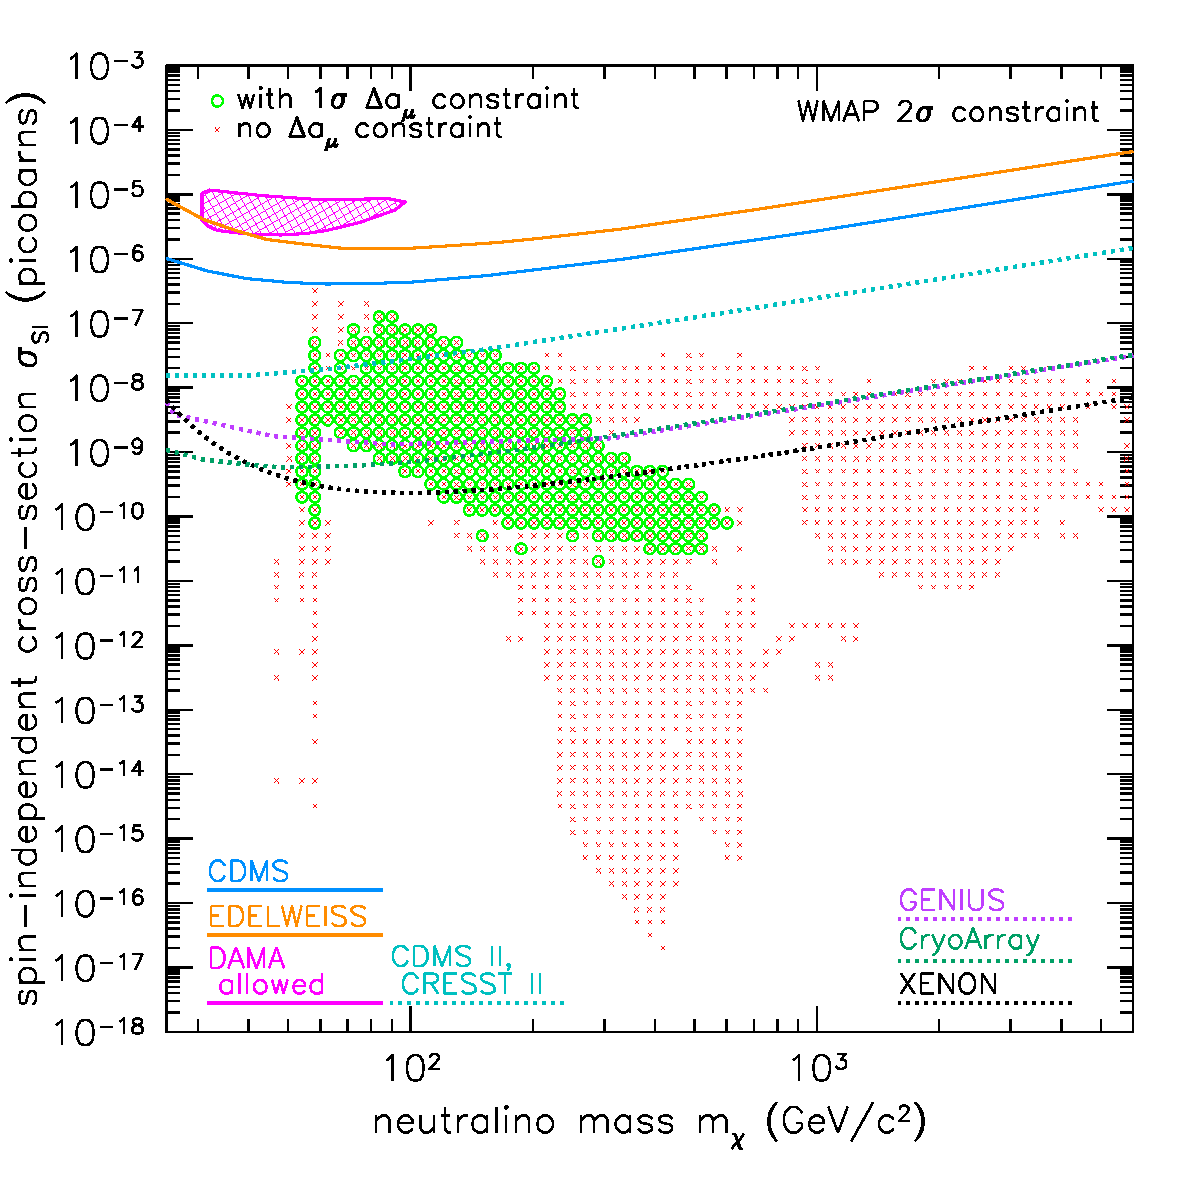
\includegraphics[width=\textwidth]{sigsi}
\column{0.5\linewidth}
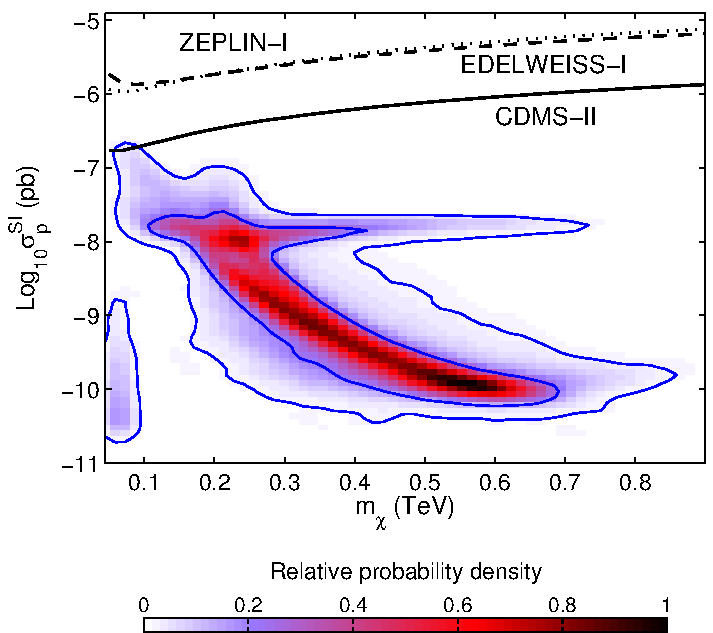
\includegraphics[width=\textwidth]{Ruiz06}
\end{columns}

\end{frame}

\begin{frame}
\frametitle{2008-09}

\begin{columns}
\column{1.05\linewidth}

\begin{itemize}
  \item MultiNest -- Faster posterior sampling (Feroz \& Hobson, Trotta et al 2008) 
  \item Improved frequentist analyses -- profile likelihood (Trotta et al 2008, Akrami, PS et al 2009, Mastercode 2009+)
\end{itemize}

\end{columns}

\vspace{2mm}

\begin{columns}
\column{0.5\linewidth}
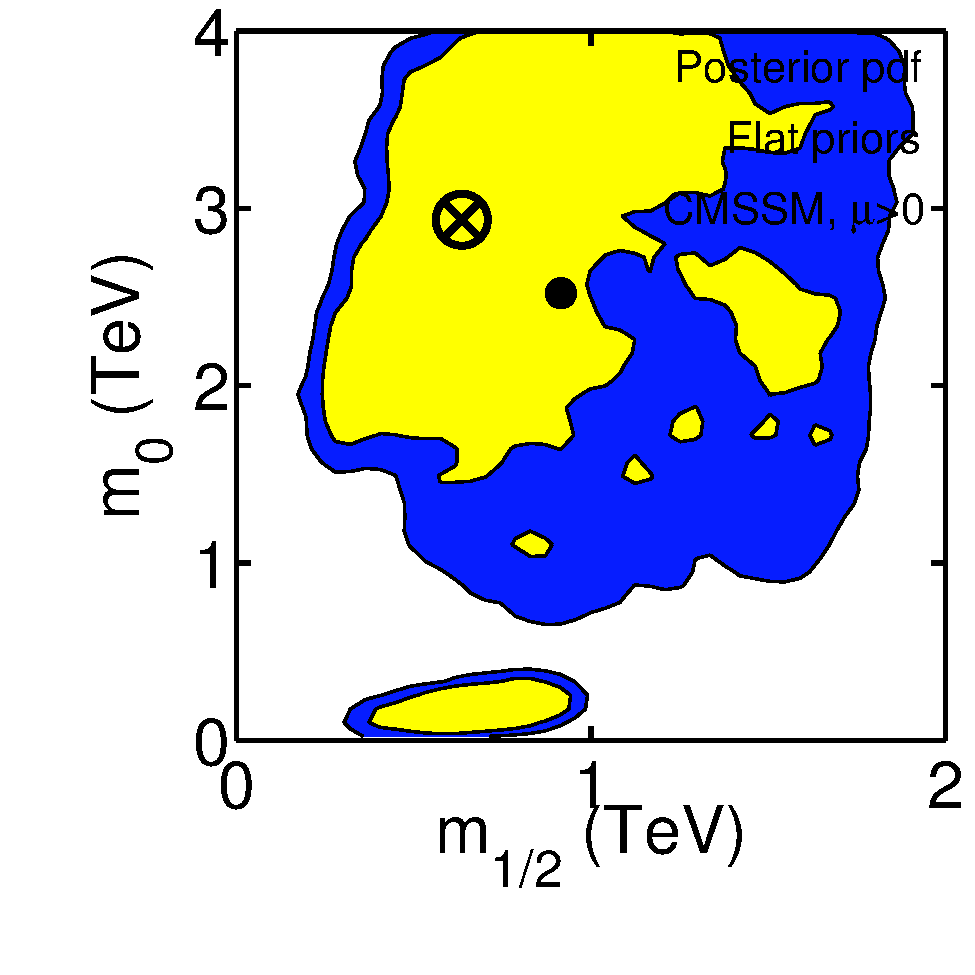
\includegraphics[width=0.9\textwidth]{Trotta08}
\column{0.5\linewidth}
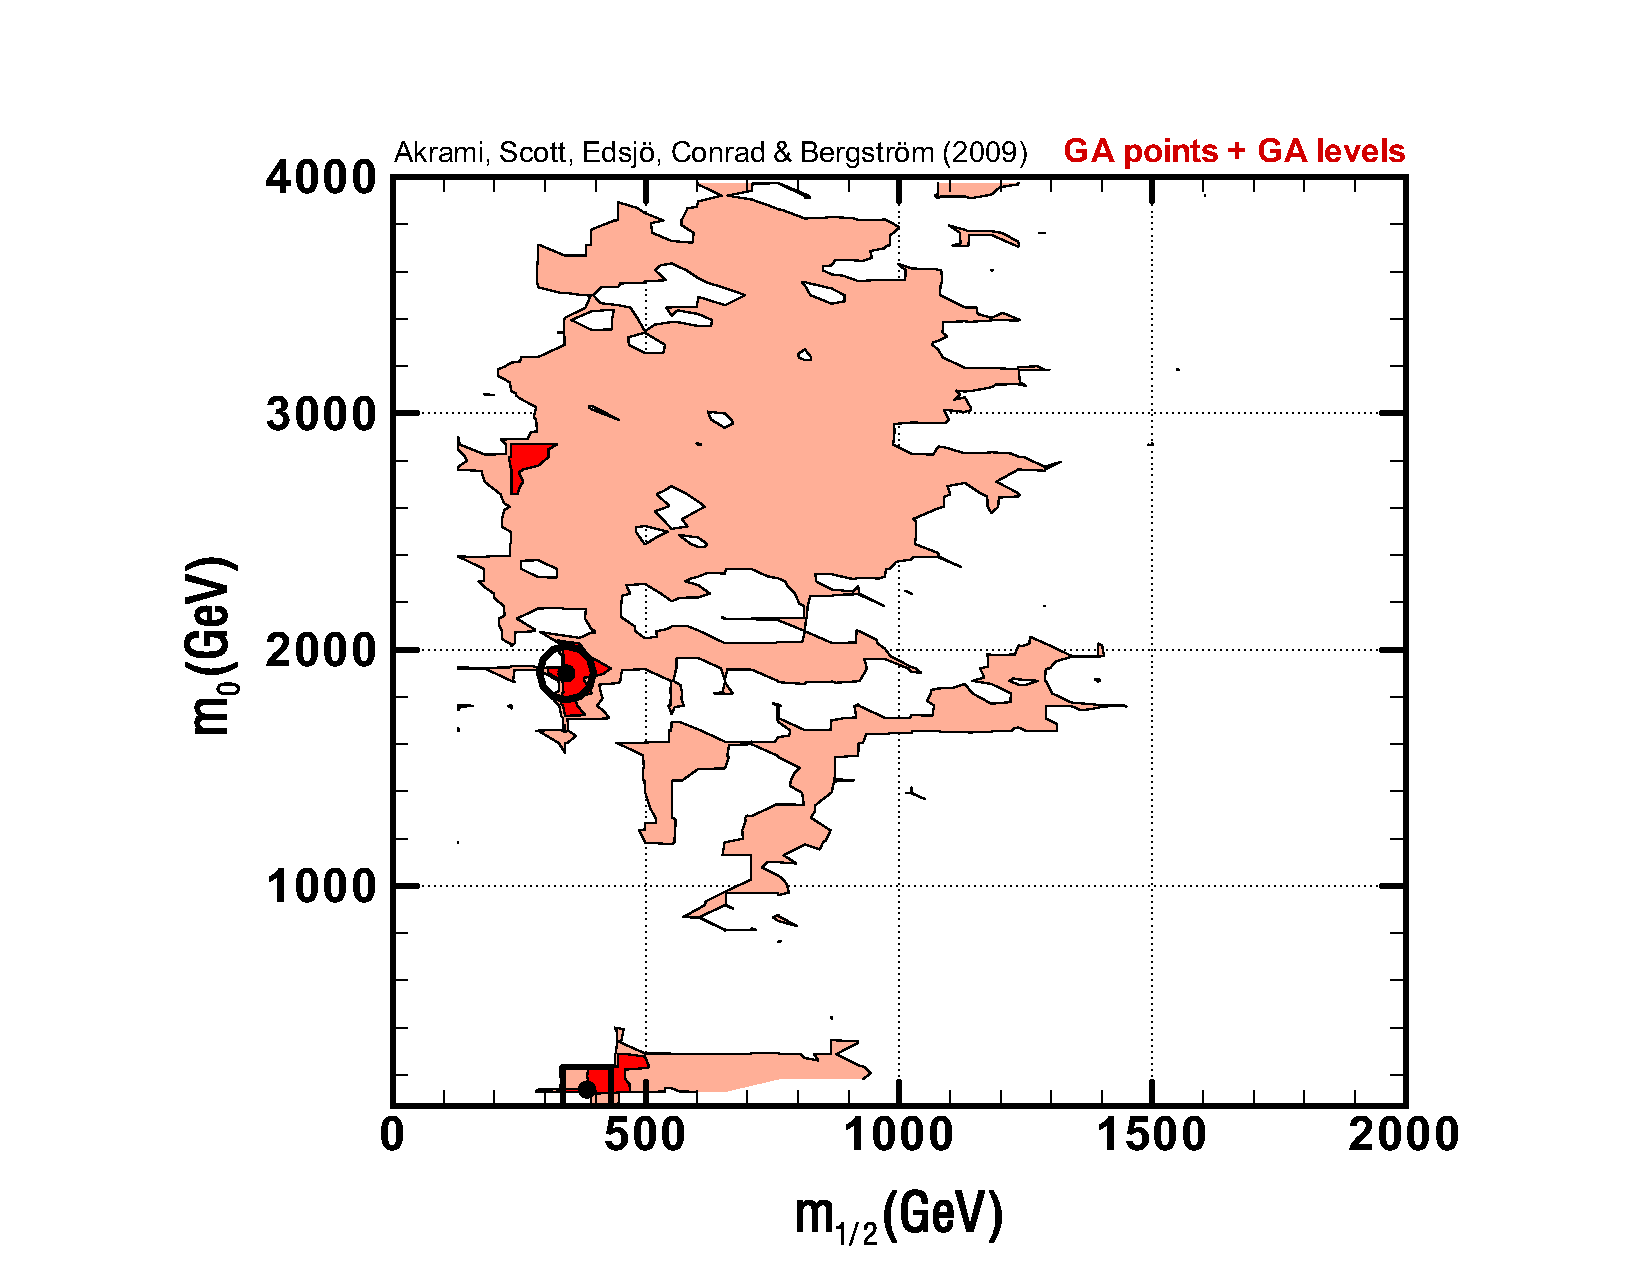
\includegraphics[width=1.1\textwidth, trim = 0 0 0 65, clip = true]{GA_m0mhf_GAlevels}
\end{columns}

\end{frame}


\begin{frame}
\frametitle{Theories/Models: Please, anything but the CMSSM!}

\begin{columns}[c]
\column{0.5\linewidth}
\begin{itemize}
\item{General low-energy SUSY\\\hspace{3mm}\footnotesize(AbdusSalam et al 2010)}
\item{Small perturbations on CMSSM:\\\hspace{3mm}\footnotesize NUHM1, NUHM2, VCMSSM\\\hspace{3mm}(Roskowski et al 2009, \\\hspace{3mm}Mastercode 2009+)}
\item{CNMSSM / NmSUGRA\\\hspace{3mm}\footnotesize Extra SM singlet + singlino\\\hspace{3mm}(Lopez-Fogliani et al 2009)}
\item{Universal Extra Dimensions\\\hspace{3mm}\footnotesize with Kaluza-Klein DM\\\hspace{3mm}(Bertone et al 2010)}
\end{itemize}
\column{0.5\linewidth}
\centering
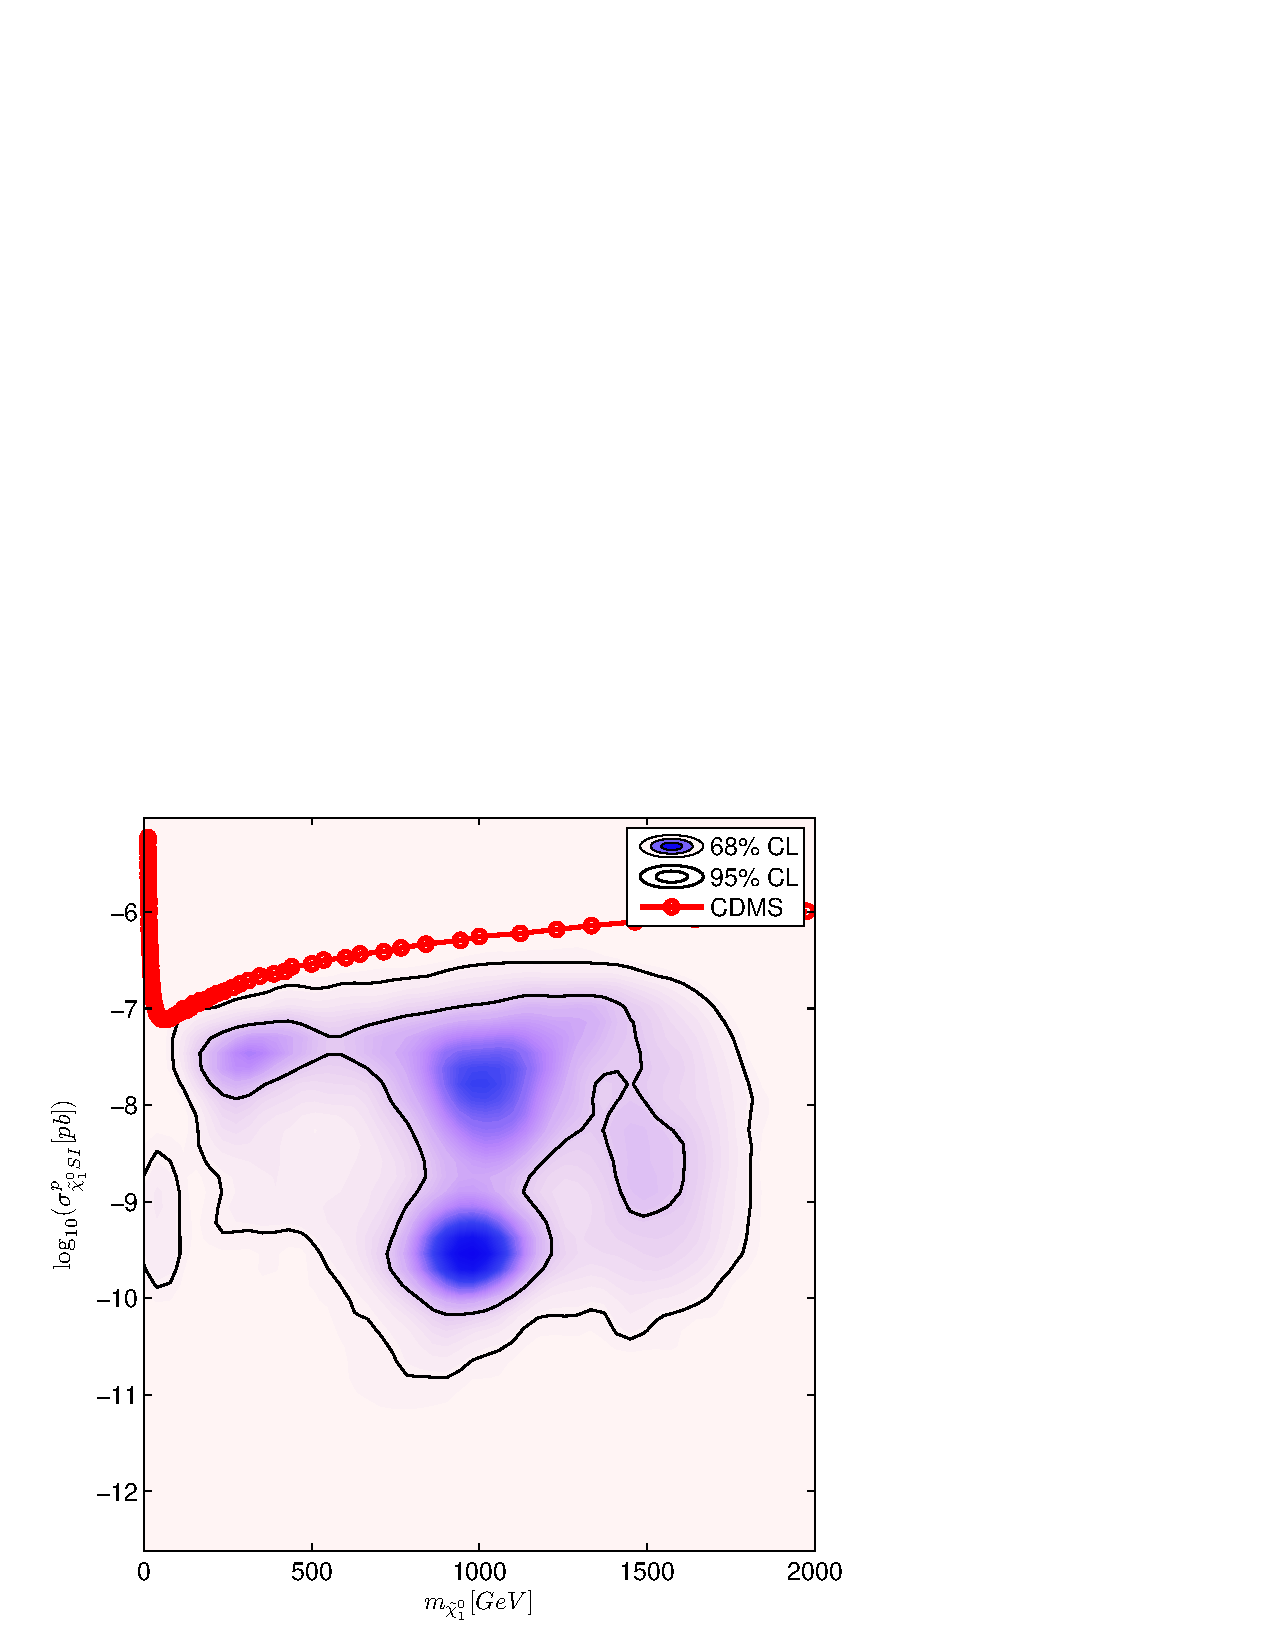
\includegraphics[width=0.73\textwidth, trim = 0 0 150 390, clip = true]{pMSSMSI}\\
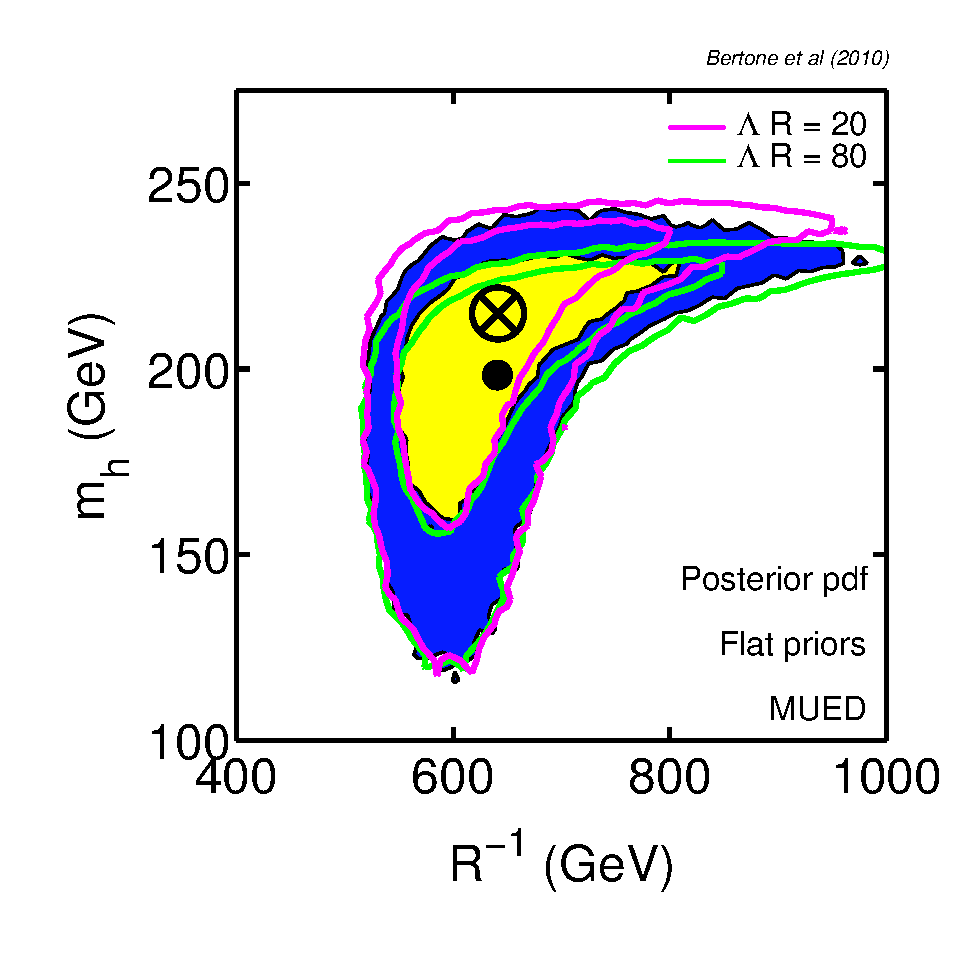
\includegraphics[width=0.82\textwidth,trim = 0 20 0 40, clip = true]{UED}\\
\end{columns}

\end{frame}


\begin{frame}
\frametitle{Addition of LHC data}

1--5 fb$^{-1}$ data, 7--8 TeV centre of mass energy (2011-12)
\begin{itemize}
  \item ATLAS/CMS LHC searches for supersymmetry 
  \item Higgs signals
\end{itemize}
\vspace{8mm}

\begin{columns}
\column{0.35\linewidth}
\centering
SuperBayes
\column{0.35\linewidth}
\centering
MasterCode
\column{0.35\linewidth}
\centering
Fittino
\end{columns}

\begin{columns}
\column{0.38\linewidth}
\centering
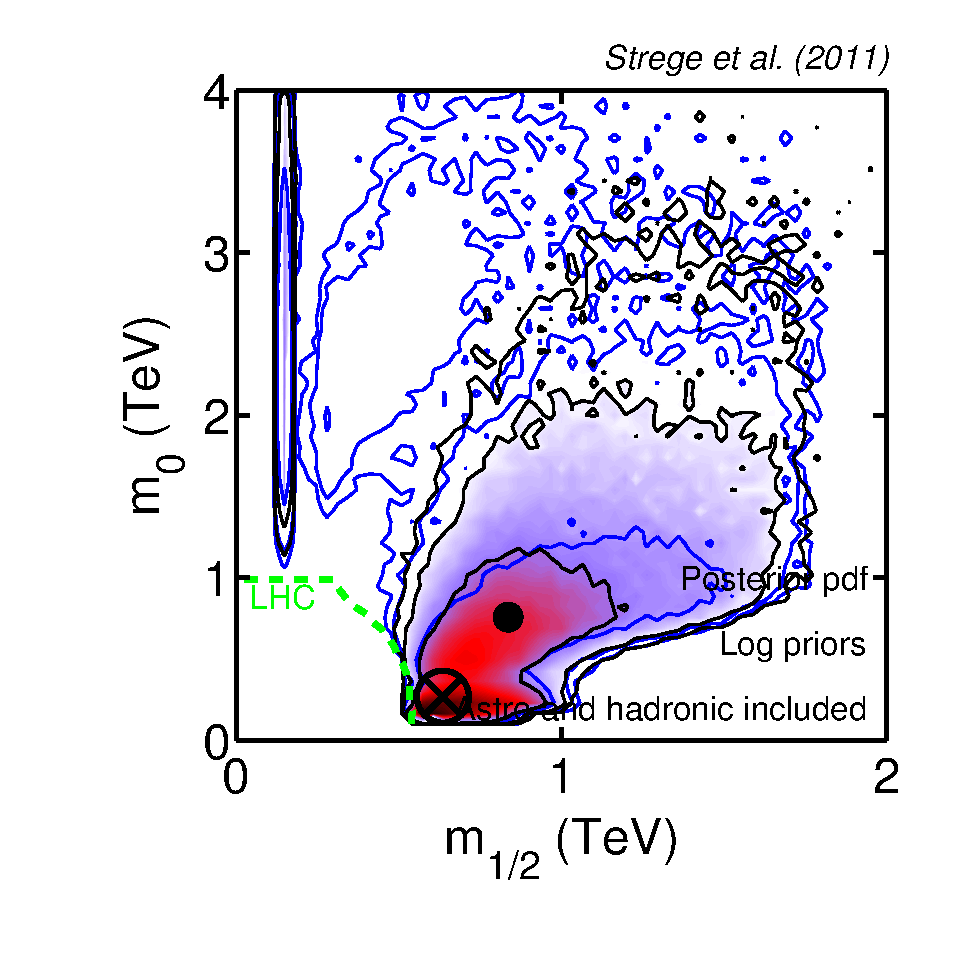
\includegraphics[width=\textwidth]{Strege11}
\column{0.38\linewidth}
\centering
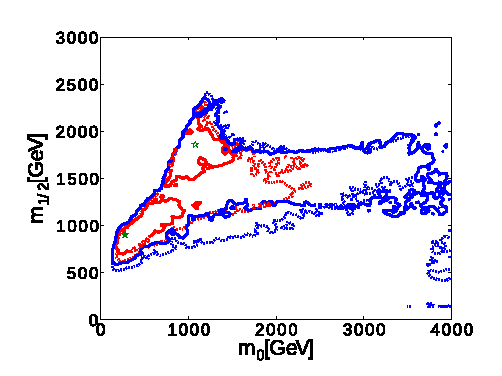
\includegraphics[width=\textwidth]{MasterCode2012_CMSSM}
\column{0.38\linewidth}
\centering
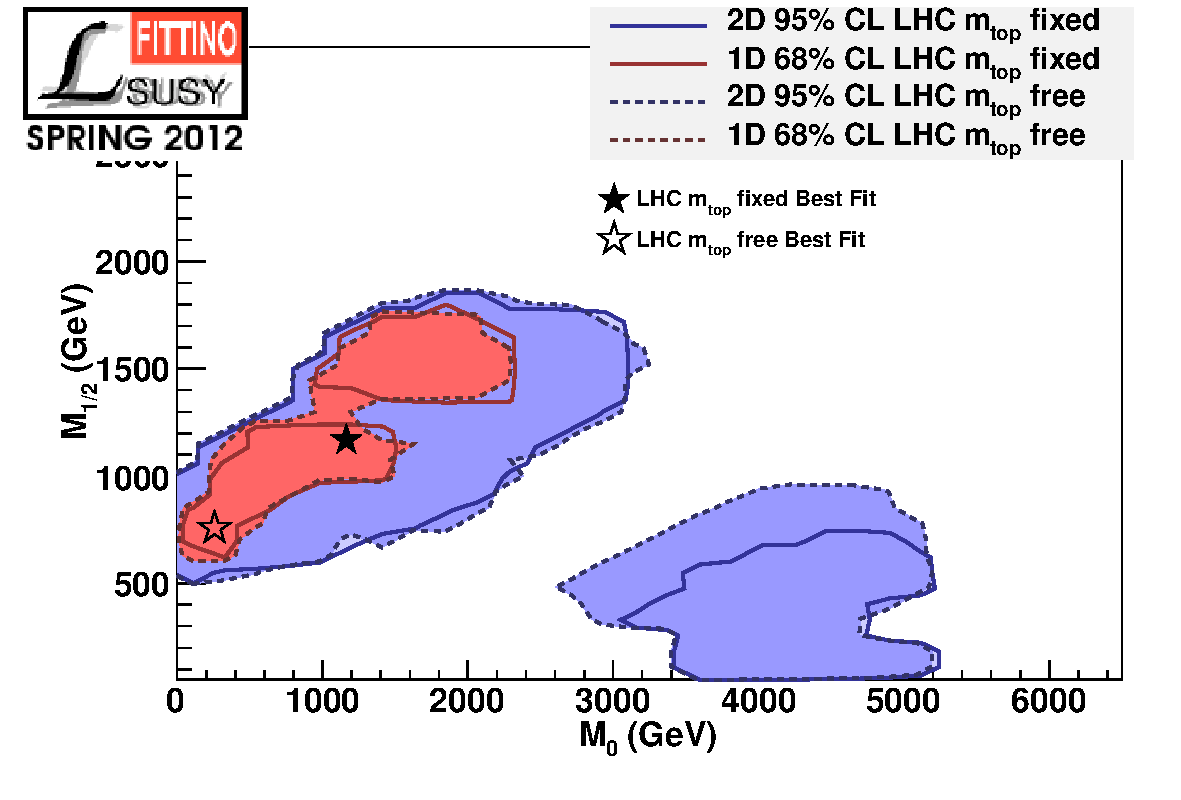
\includegraphics[width=\textwidth]{Fittino}
\end{columns}

\end{frame}


\subsection{Indirect detection of dark matter}

\begin{frame}
\frametitle{Gamma-rays}

Gammay-ray annihilation searches have been added to the global fits: 
\vspace{3mm}

\begin{columns}[t]

\column{0.55\linewidth}
\cblue{\textit{Fermi}-LAT}

{\footnotesize
Satellite pair conversion telescope

Dwarf galaxy Segue 1

(PS, Conrad et al 2009)
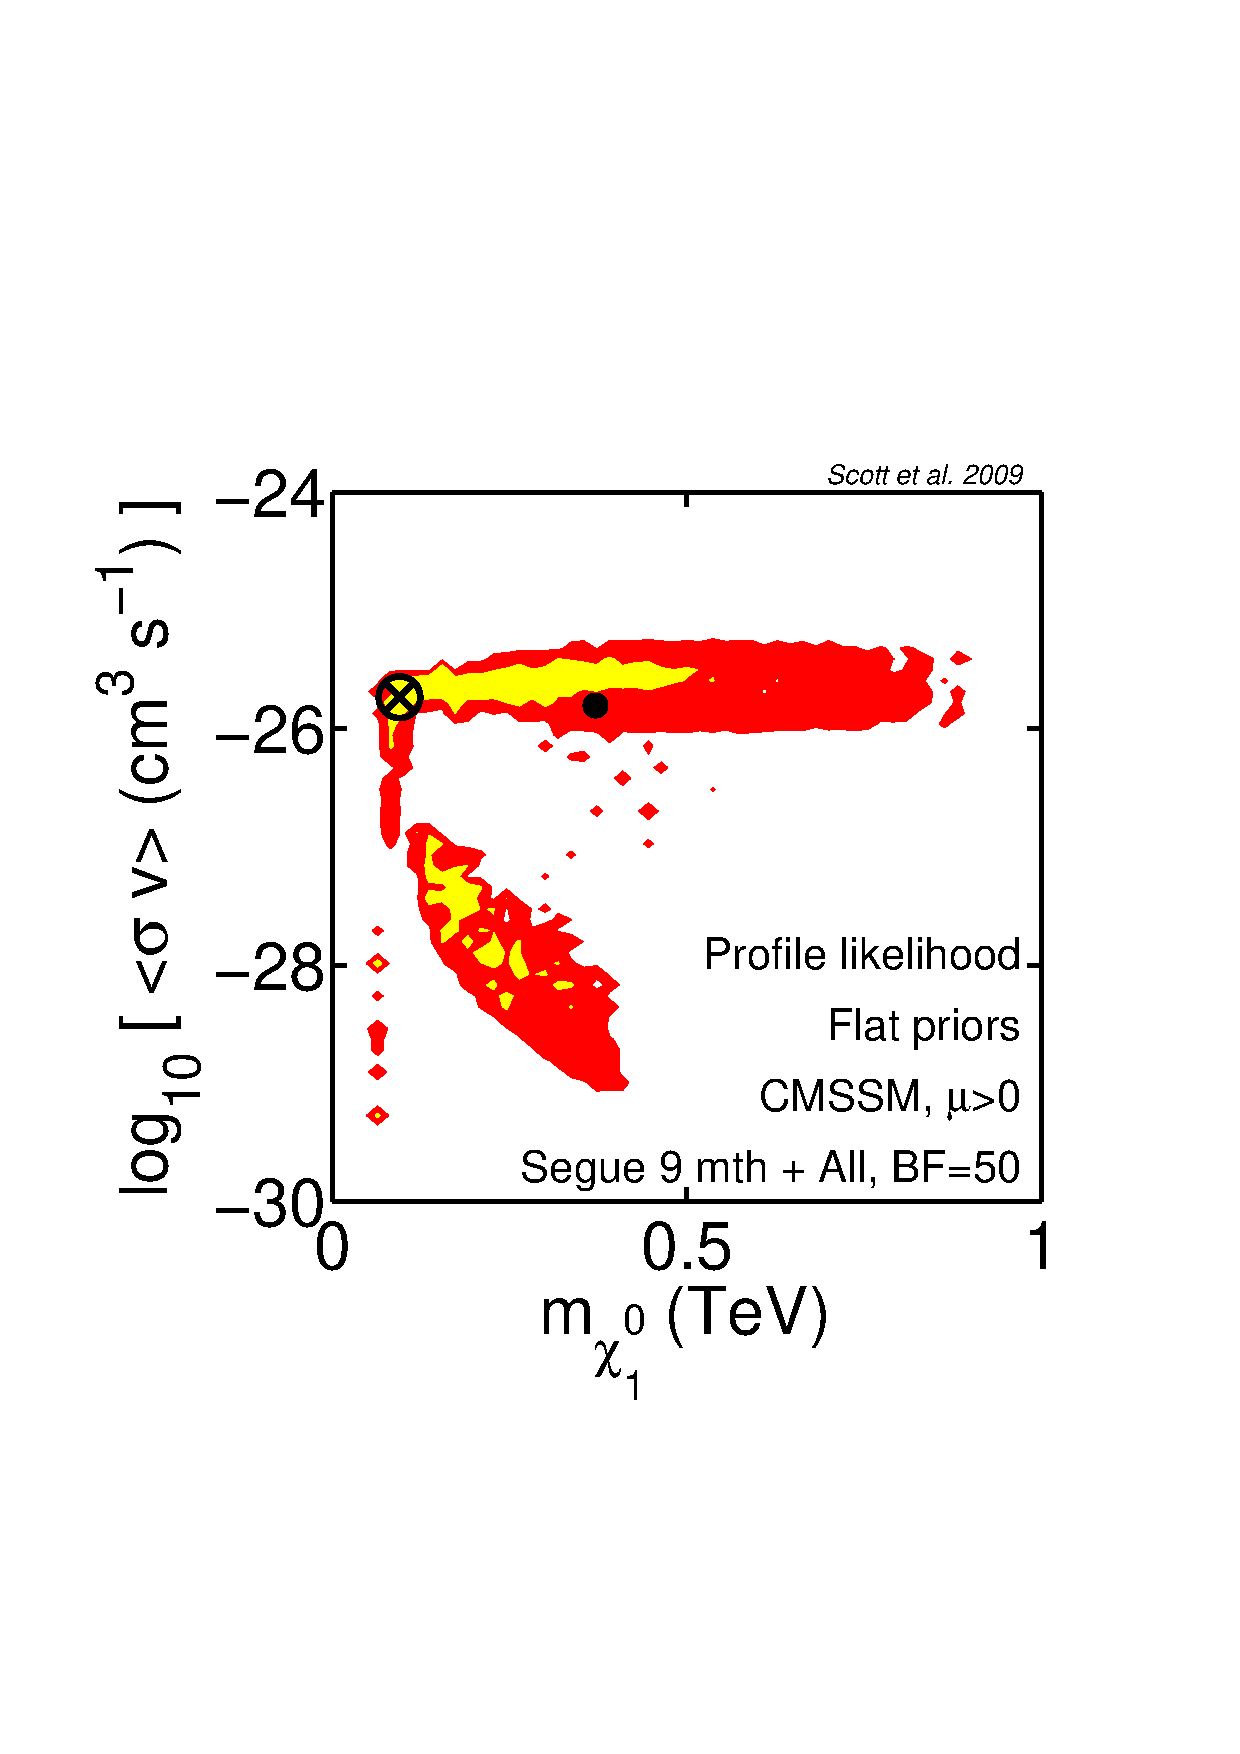
\includegraphics[width=0.9\textwidth, trim = 0 0 0 200, clip=true]{B50_H0_All_P_lin_2D_profl_7}
}

\column{0.55\linewidth}
\cblue{HESS}

{\footnotesize
Air \v{C}erenkov telescope

Milky Way$+$Carina$+$Sculptor$+$Sag dwarf

(Ripken, Conrad \& PS 2011)\vspace{2mm}

\only<1>{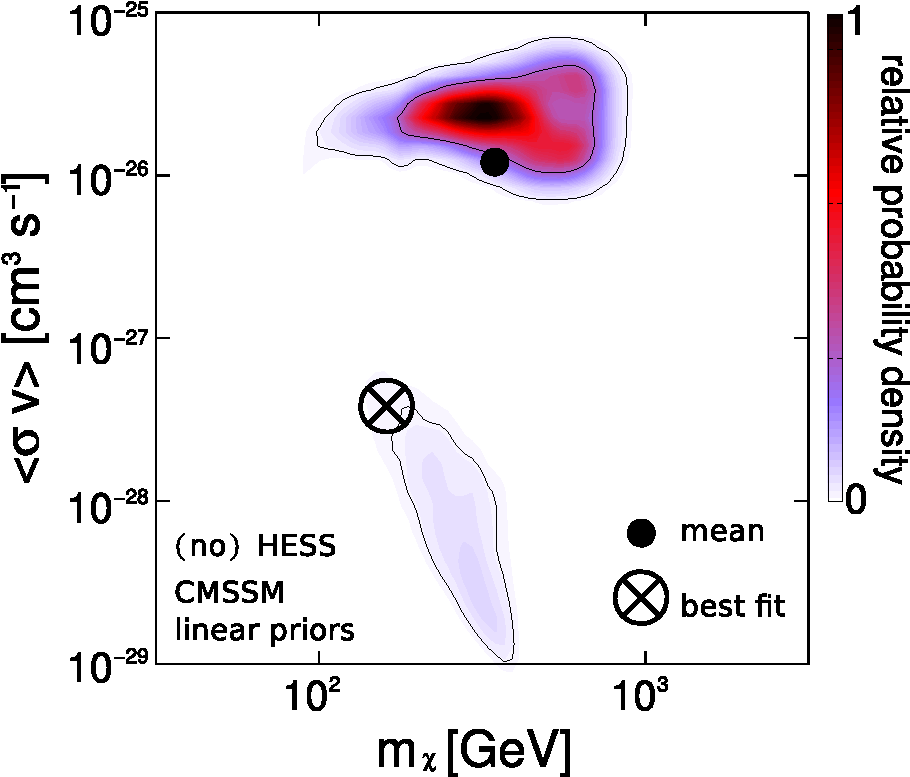
\includegraphics[width=0.8\textwidth]{noHESS}}%
\only<2>{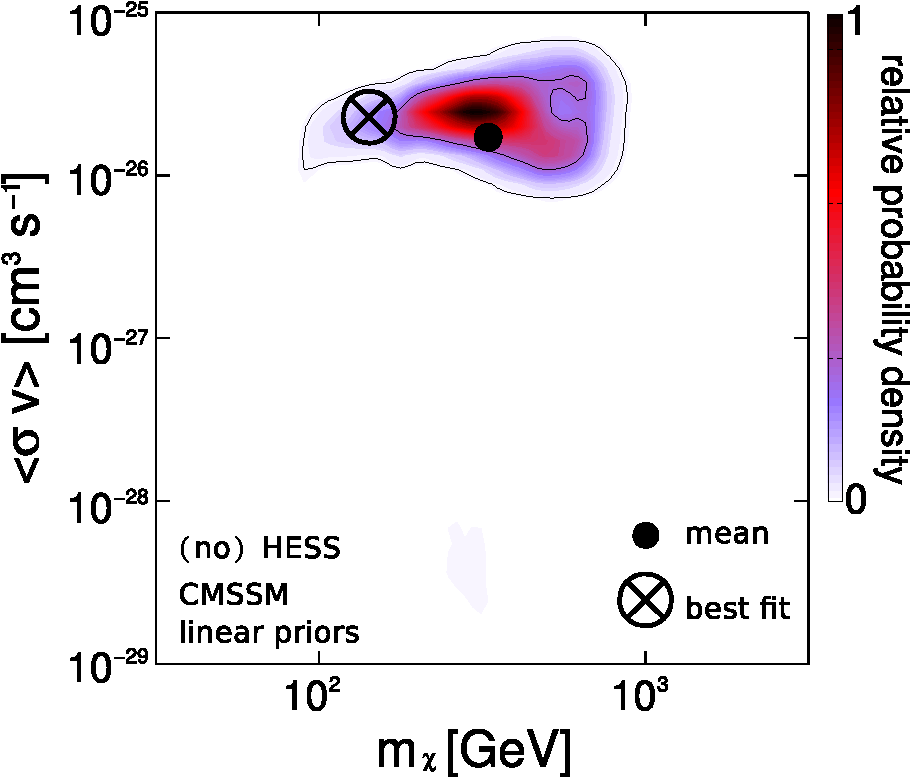
\includegraphics[width=0.8\textwidth]{allHESS}}
}

\end{columns}

\end{frame}


\begin{frame}
\frametitle{Neutrinos}

New likelihood analysis including IceCube Neutrino Telescope WIMP-search neutrino events
\vspace{3mm}

\begin{columns}[t]
\column{0.58\linewidth}
\cblue{IceCube 22-string data}\\
{\footnotesize
Not expected to be very constraining\\
\visible<2->{\ldots but at least we know it works}\\
(PS, Savage, Edsj\"o \& IceCube Collab 2012)
\only<1,3-4>{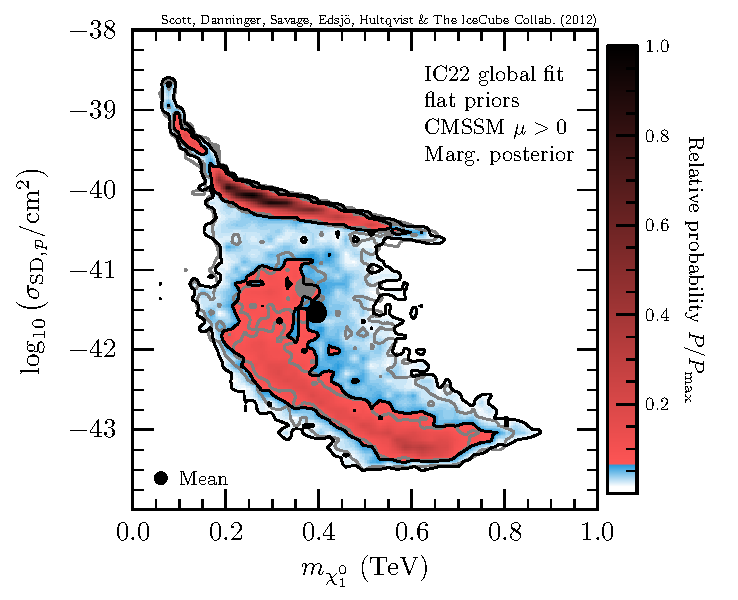
\includegraphics[width=0.85\textwidth]{IC22_marg3}}%
\only<2>{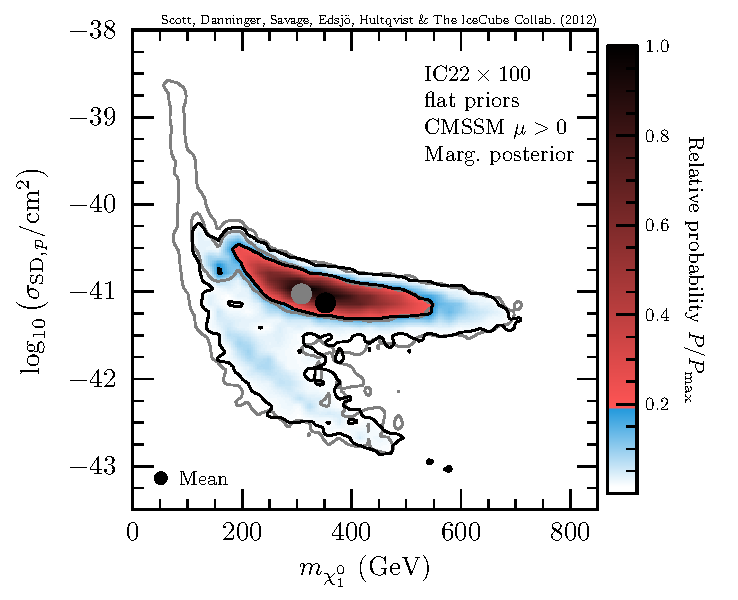
\includegraphics[width=0.85\textwidth]{recon2D_4}}
}
\column{0.58\linewidth}
\visible<3->{%
\cblue{IceCube-DeepCore (86-string)}\\
{\footnotesize
Very constraining (projection)
\visible<4>{$\implies$ unique access to pts in more general MSSM}\\
\visible<4>{(Silverwood, PS, Danninger et al 2012)}
\only<3>{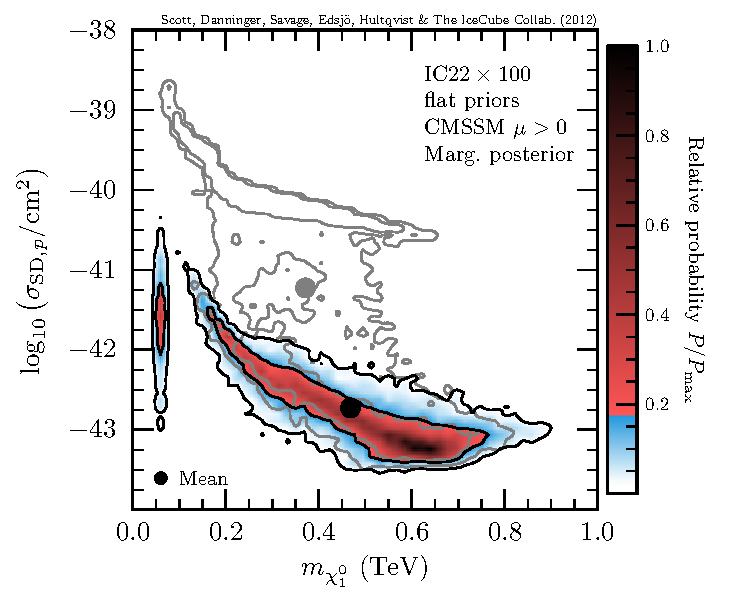
\includegraphics[width=0.85\textwidth]{IC22x100_marg3}}%
\only<4>{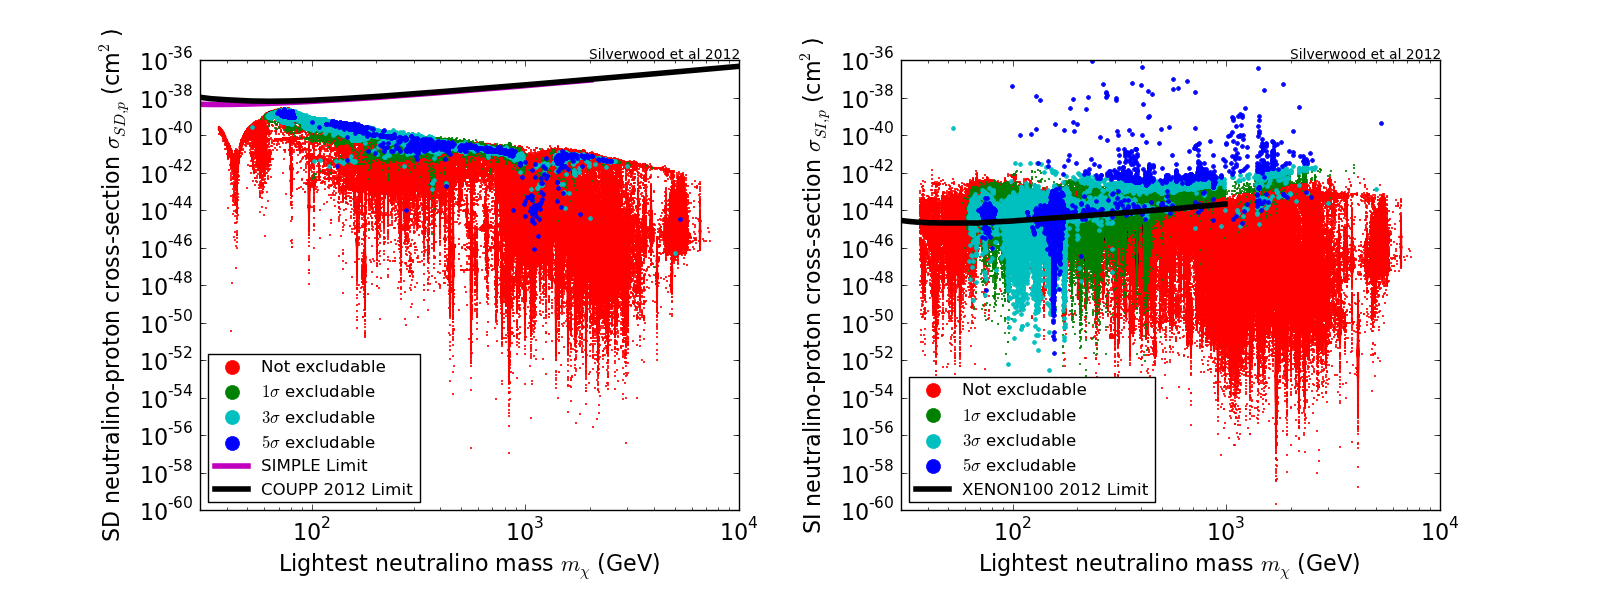
\includegraphics[width=0.9\textwidth, trim = 550 0 0 0, clip=true]{MSSM25}}
}}
\end{columns}


\end{frame}



\subsection{Direct detection of dark matter}

\begin{frame}
\frametitle{Direct detection data in global fits}
XENON-100 bounds now maybe starting to impact BSM theories (Strege et al 2011, Mastercode 2011+, Fittino 2012)\\
  {\footnotesize\hspace{3mm}-- depends strongly on hadronic uncertainties}
\vspace{2mm}

Tonne-scale detection could allow us to zoom in very quickly on the correct parameters (Akrami, Savage, PS et al 2011b)
\vspace{2mm}

\begin{columns}
\column{1.05\linewidth}
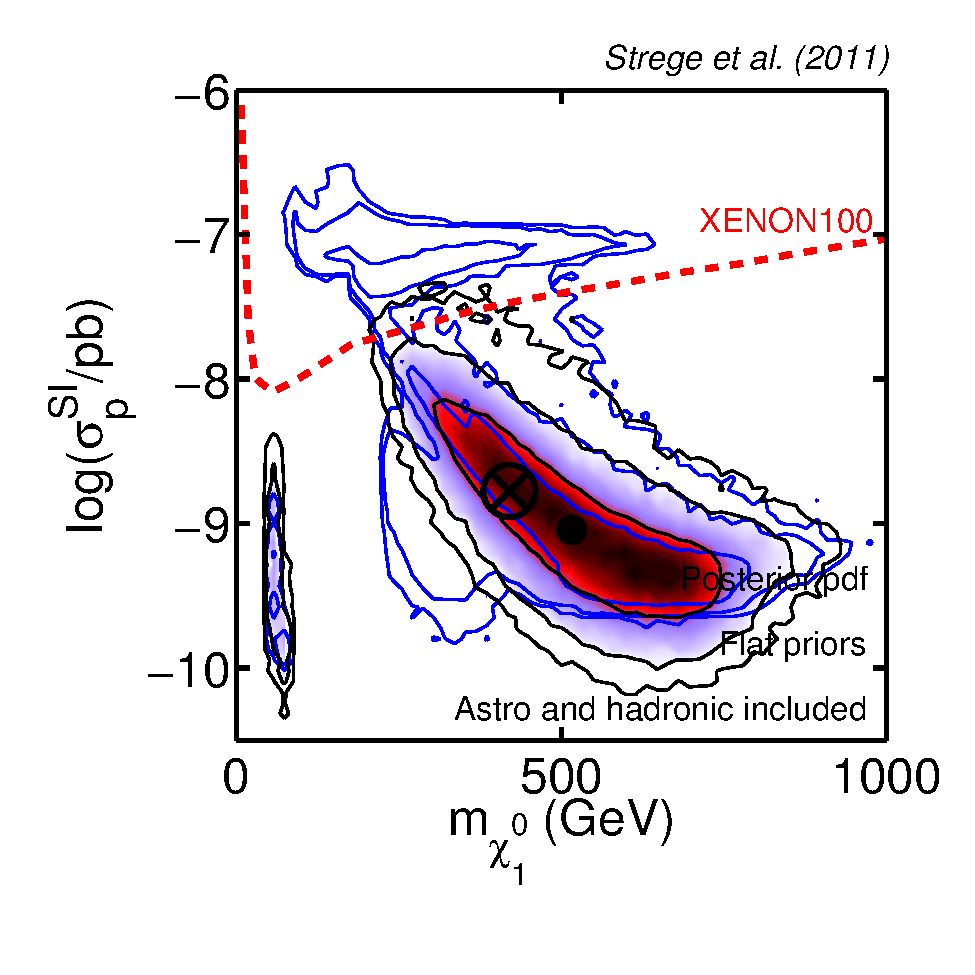
\includegraphics[width=0.33\textwidth]{Strege11_DD}\hspace{3mm}
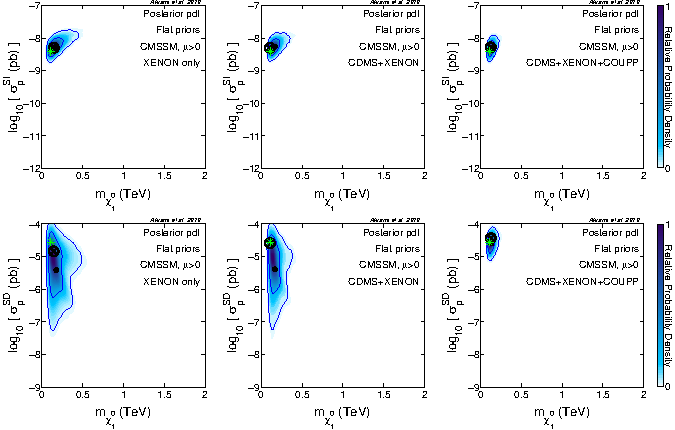
\includegraphics[width=0.62\textwidth]{DD_DDparams}
\end{columns}

\end{frame}

\begin{frame}
\frametitle{Combined Direct + Indirect + LHC constraints}

\Large

\visible<1-4>{Base Observables} \visible<2-4>{$+$ XENON-100} \visible<3-4>{$+$ CMS\,5\,fb$^{-1}$}

{\centering \visible<4>{$+$ IC22$\times$100}}

\vspace{2mm}
\footnotesize
\visible<2-4>{Grey contours correspond to Base Observables \textit{only}}
\vspace{2mm}

\begin{columns}
\column{0.36\textwidth}
\only<1>{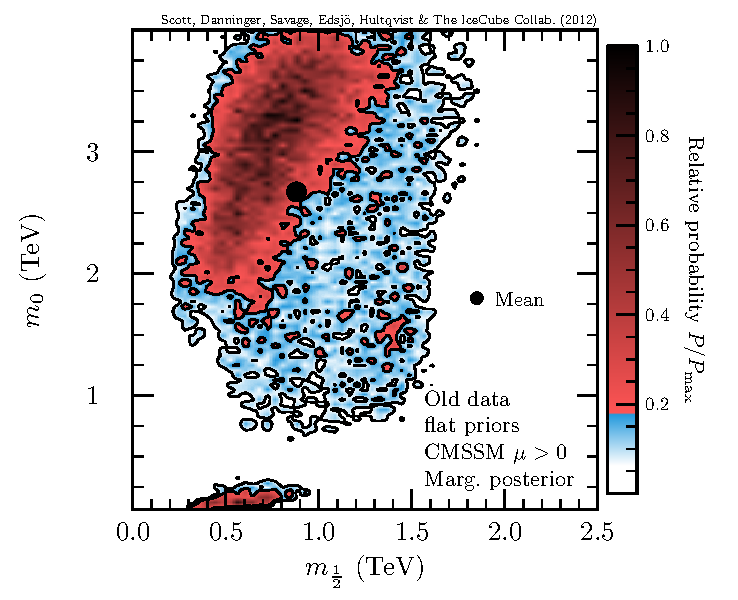
\includegraphics[height=0.92\linewidth, trim = 8 0 30 0, clip = true]{marg2D_1_1}}%
\only<2>{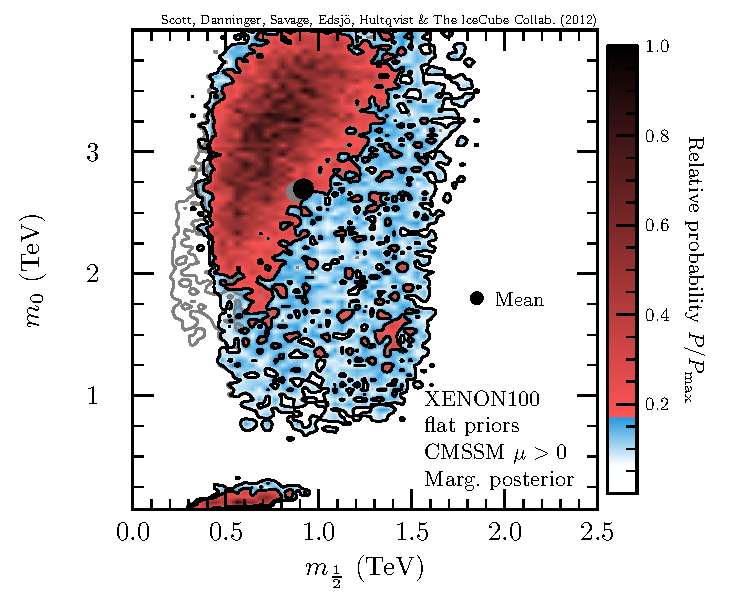
\includegraphics[height=0.92\linewidth, trim = 8 0 30 0, clip = true]{marg2D_2_1}}%
\only<3>{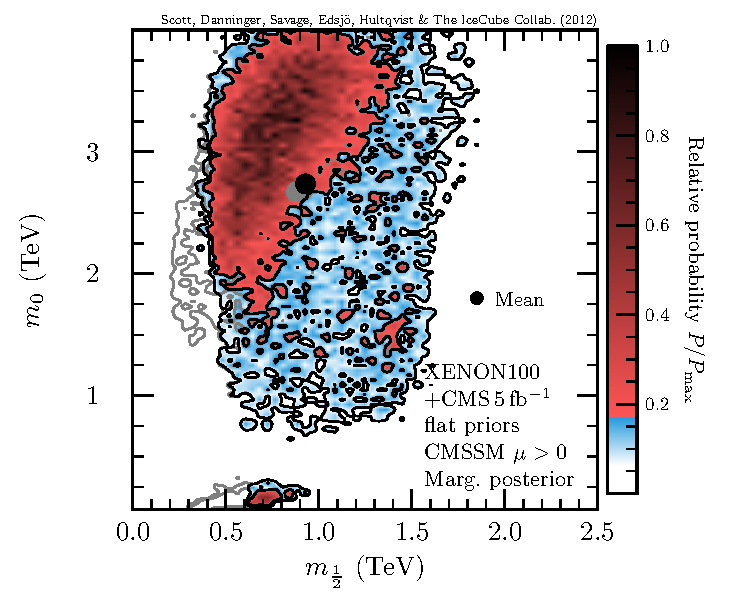
\includegraphics[height=0.92\linewidth, trim = 8 0 30 0, clip = true]{marg2D_3_1}}%
\only<4>{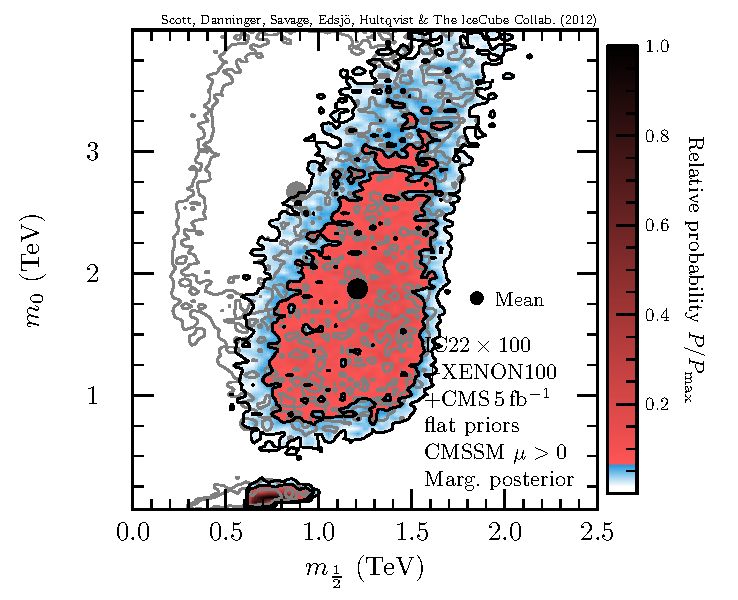
\includegraphics[height=0.92\linewidth, trim = 8 0 30 0, clip = true]{marg2D_4_1}}
\column{0.36\textwidth}
\only<1>{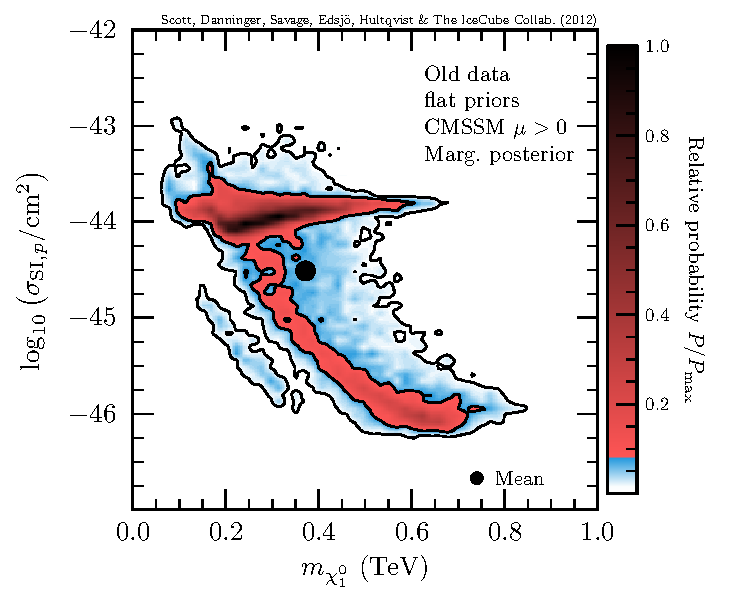
\includegraphics[height=0.92\linewidth, trim = 8 0 30 0, clip = true]{marg2D_1_2}}%
\only<2>{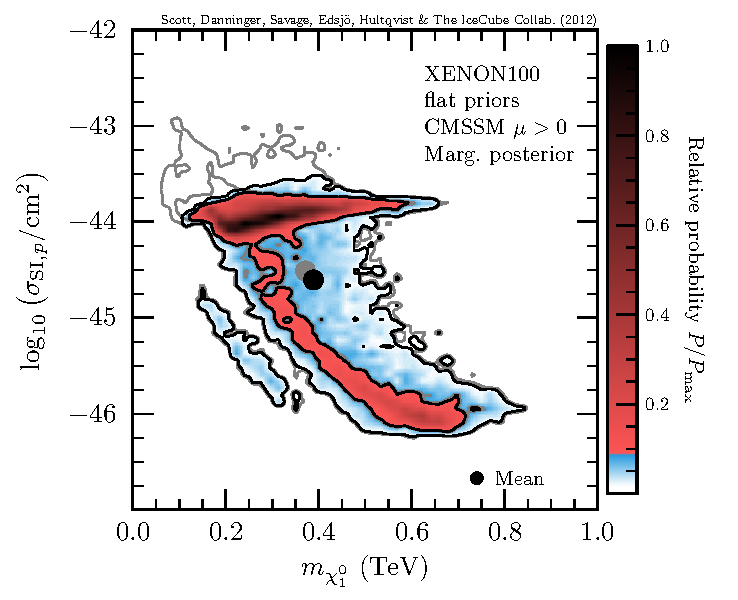
\includegraphics[height=0.92\linewidth, trim = 8 0 30 0, clip = true]{marg2D_2_2}}%
\only<3>{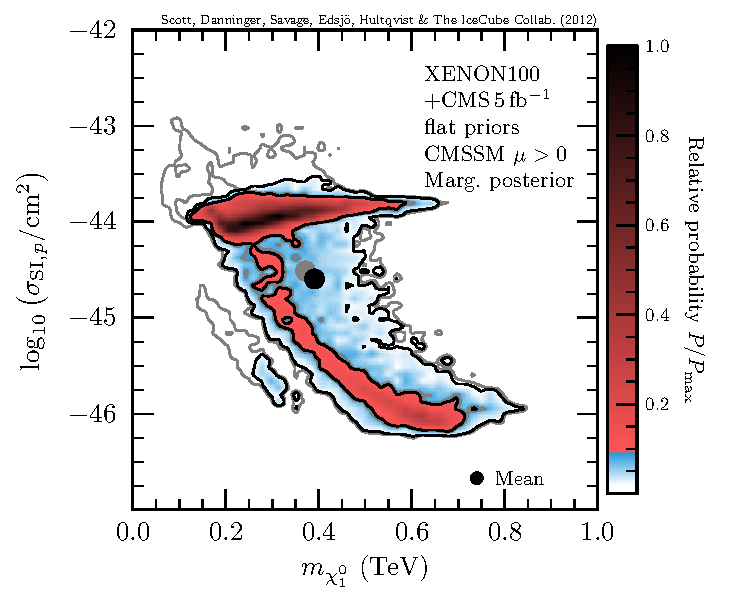
\includegraphics[height=0.92\linewidth, trim = 8 0 30 0, clip = true]{marg2D_3_2}}%
\only<4>{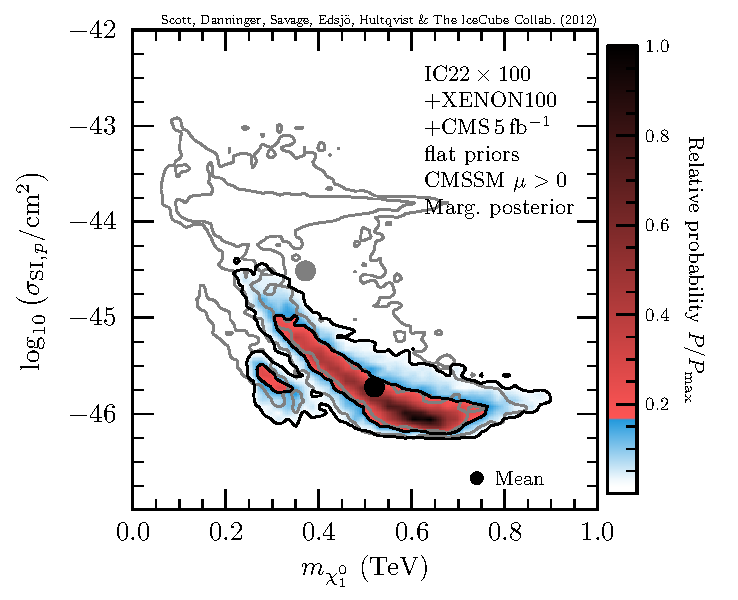
\includegraphics[height=0.92\linewidth, trim = 8 0 30 0, clip = true]{marg2D_4_2}}
\column{0.36\textwidth}
\only<1>{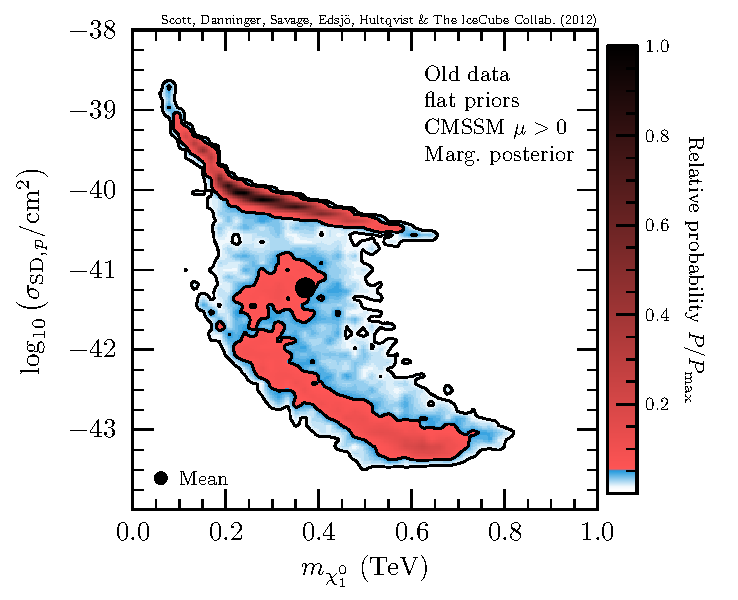
\includegraphics[height=0.92\linewidth, trim = 8 0 10 0, clip = true]{marg2D_1_3}}%
\only<2>{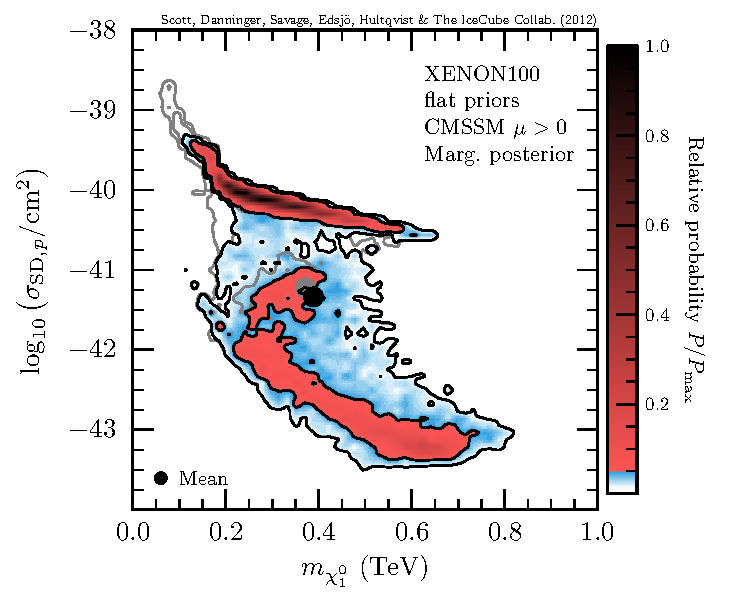
\includegraphics[height=0.92\linewidth, trim = 8 0 10 0, clip = true]{marg2D_2_3}}%
\only<3>{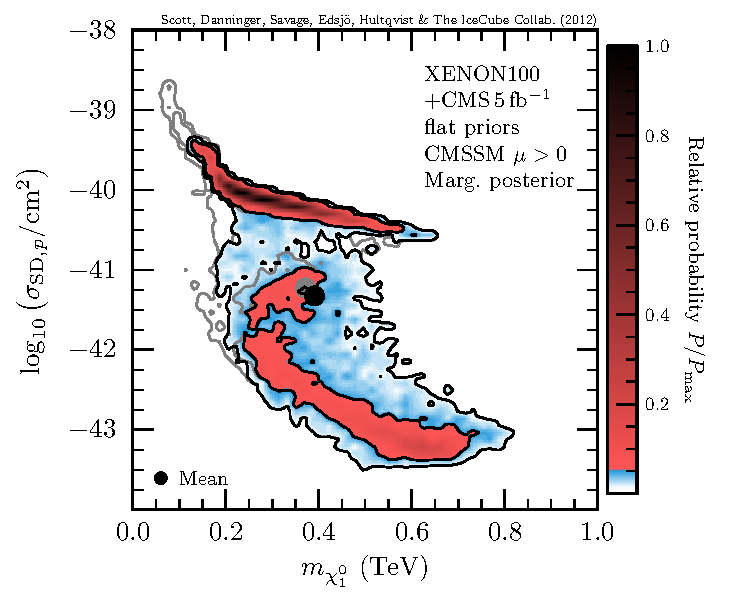
\includegraphics[height=0.92\linewidth, trim = 8 0 10 0, clip = true]{marg2D_3_3}}%
\only<4>{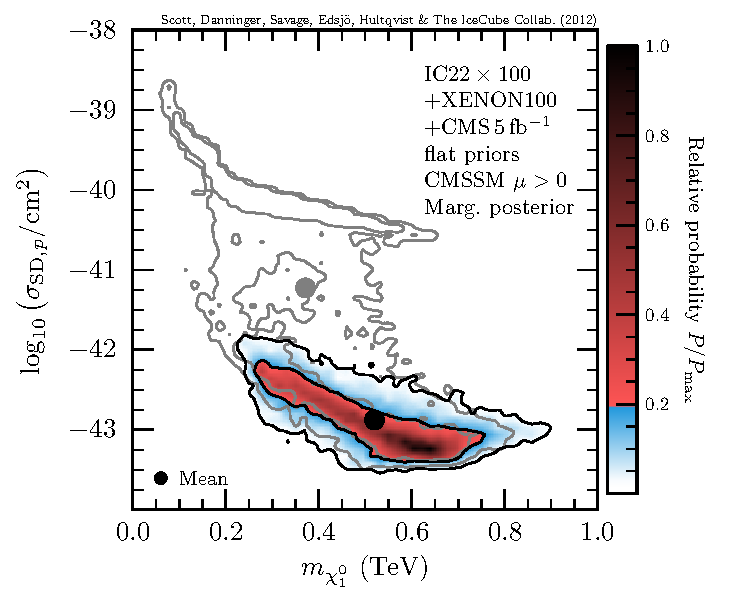
\includegraphics[height=0.92\linewidth, trim = 8 0 10 0, clip = true]{marg2D_4_3}}
\end{columns}
\vspace{2mm}

\visible<4>{\textbf{CMSSM, IceCube-22 with 100$\times$ boosted effective area}\\
(kinda like IceCube-DeepCore)}

\end{frame}

\section{Future Challenges}

\subsection{Respectable LHC and astro likelihoods}

\begin{frame}
\frametitle{Getting LHC data into global fits}

Typical workflow in a collider phenomenology analysis:

\begin{enumerate}
\item Choose your new symmetries or effective operators
\item Augment SM Lagrangian with new terms
\item Derive Feynman rules
\item Derive/calculate cross-sections
\item Simulate events -- parton showering
\item Simulate events -- hadronisation
\item Rescale rates due to neglected loops (or other reasons)
\item Do `fast' detector simulation of events to get final predicted rate
\item Repeat steps 5-8 for each point in parameter space
\end{enumerate}

\end{frame}

\begin{frame}
\frametitle{The LHC monster}

\visible<1->{
\begin{exampleblock}{Time per point:}
$\mathcal{O}(minute)$ in \alert{best} cases
\end{exampleblock}
}

\visible<2->{
\begin{exampleblock}{Time per point for global fits to converge:}
$\mathcal{O}(seconds)$ in \alert{worst} cases
\end{exampleblock}
}

\visible<3->{
\begin{exampleblock}{Challenge:}
About 2 orders of magnitude too slow to actually include LHC data in global fits properly
\end{exampleblock}
}

\end{frame}

\begin{frame}
\frametitle{Taming the LHC monster}

\only<1,2>{
\begin{exampleblock}{Zeroth Order Response:}
``Stuff it, just use the published limits and ignore the dependence on other parameters''
\end{exampleblock}

\visible<2>{
\vspace{5mm}
Obviously naughty -- plotted limits assume CMSSM, and fix two of the parameters
\begin{itemize}    
  \item Don't really know dependence on other parameters
  \item Don't have a likelihood function, just a line
  \item Can't use this at all for non-CMSSM global fits -- e.g. MSSM-25
\end{itemize}

\vspace{5mm}
Those in the room having done this can remain unidentified \smiley
}}  

\only<3,4>{
\begin{exampleblock}{First Order Response:}
``Test if things depend on the other parameters (hope not), re-simulate published exclusion curve''
\end{exampleblock}

\visible<4>{
\vspace{5mm}
Not that great, but OK in some cases
\begin{itemize}    
  \item At least have some sort of likelihood this time
  \item Still a bit screwed if things do depend a lot on other parameters, but
  \item allows (potentially shaky) extrapolation, also to non-CMSSM models
\end{itemize}

\vspace{5mm}
Fittino, Mastercode
}}

\only<5,6>{
\begin{exampleblock}{Negative Order Response:}
``I am such an \"ubersmart particle theorist that I know much more about statistics than all those silly experimentalists and global fitters put together.\\\vspace{2mm}``I'll just do an undersampled random scan and count the points, that way I don't need to worry about all this sampling/statistics nonsense!''
\end{exampleblock}

\visible<6>{
\vspace{5mm}
(Sadly, people do think like this -- and continue to publish such papers.  I fight with them at meetings.)
}}

\only<7,8>{
\begin{exampleblock}{Second Order Response:}
``That's ridiculous.  I've never met a calculation I can't speed up.  There must be some way to have my cake and eat it too''
\end{exampleblock}

\visible<8>{
\vspace{5mm}
Maybe -- this is the challenge.
\begin{itemize}    
  \item Interpolated likelihoods (how to choose nodes?)
  \item Neural network functional approximation (how to train accurately?)
  \item Some sort of smart reduction based on event topology? 
  \item Something else?
\end{itemize}
}}

\end{frame}

\begin{frame}
  \frametitle{Two different approaches to including astro data in BSM scans}

  \begin{enumerate}
  \item{Just use the published limits on $\langle \sigma v\rangle$ (or $\sigma_\mathrm{SI,SD}$)}
    \begin{itemize}
    \item{Fast -- can cover large parameter spaces}
    \item{Not so accurate -- experimental limits are invariably based on theoretical assumptions, e.g. $b\bar b$ spectrum}
    \item{Full likelihood function almost never available}
    \end{itemize}
  \item\alert<2-3>{Use the data points directly in SUSY scans} 
    \begin{itemize}
    \item{Slow -- requires full treatment of instrument profile for each point}
    \item{Accurate -- can test each point self-consistently}
    \item{Allows marginalisation over theoretical assumptions}
    \item{Allows construction of full multi-dimensional likelihood function}
    \end{itemize}
  \visible<3>{\item\alert{(indirect only: use just flux upper limits)}}
  \end{enumerate}

\end{frame}

\begin{frame}
\frametitle{Example: Advanced IceCube Likelihood (Part 1)}

Simplest way to do anything is to make it a counting problem\ldots
\vspace{5mm}

Compare observed number of events $n$ and predicted number $\theta$ for each model, taking into account error $\sigma_\epsilon$ on acceptance:

\begin{equation}
\label{fancy}
\scriptsize
\Like_\mathrm{num}(n|\theta_\mathrm{BG}+\theta_\mathrm{sig}) = \frac{1}{\sqrt{2\pi}\sigma_\epsilon}\int_0^\infty \frac{(\theta_\mathrm{BG}+\epsilon\theta_\mathrm{sig})^{n}e^{-(\theta_\mathrm{BG}+\epsilon\theta_\mathrm{sig})}}{n!}\frac1\epsilon\exp\left[-\frac{1}{2}\left(\frac{\ln\epsilon}{\sigma_\epsilon}\right)^2\right]\mathrm{d}\epsilon \, .
\end{equation}

\vspace{3mm}
Nuisance parameter $\epsilon$ takes into account systematic errors on effective area, from theory, etc.  $\sigma_\epsilon\sim20\%$ for IceCube.

\end{frame}

\begin{frame}
\frametitle{Example: Advanced IceCube Likelihood (Part 2)}

Full unbinned likelihood with number ($\Like_\mathrm{num}$), spectral ($\Like_\mathrm{spec}$) and angular ($\Like_\mathrm{ang}$) parts 
\begin{equation}
\footnotesize
\Like = \Like_\mathrm{num}(n|\theta_{\mathrm{signal+BG}})\prod_{i=1}^{n} \Like_{\mathrm{spec},i}\,\Like_{\mathrm{ang},i}
\end{equation}

with
\begin{equation}
\footnotesize
\Like_{\mathrm{spec},i}(\alert<2-3>{N_i}, \corangewhen{\params}{<3>}) = \frac{\theta_\mathrm{BG}}{\theta_\mathrm{signal+BG}}\cgreenwhen{\frac{dP_\mathrm{BG}}{d\alert<2-3>{N_i}}(\alert<2-3>{N_i})}{<6>} +\frac{\theta_\mathrm{signal}}{\theta_\mathrm{signal+BG}}\int_0^\infty \corangewhen{E_\mathrm{disp}(\alert<2-3>{N_i}|\Eobsi)}{<5-6>}\cbluewhen{\frac{dP_\mathrm{signal}}{d\Eobsi}(\Eobsi, \corangewhen{\params}{<3>})}{<4-6>} \,d \Eobsi
\end{equation}

and
\begin{equation}
\footnotesize
\Like_{\mathrm{ang},i}(\cgreenwhen{\cos\phi_i}{<7>}) = \frac{\theta_\mathrm{BG}}{\theta_\mathrm{signal+BG}}\cgreenwhen{\frac{dP_\mathrm{BG}}{d\cgreenwhen{\cos\phi_i}{<7>}}(\cgreenwhen{\cos\phi_i}{<7>})}{<10>} + \frac{\theta_\mathrm{signal}}{\theta_\mathrm{signal+BG}}\corangewhen{PSF(\cgreenwhen{\cos\phi_i}{<7>}|\cbluewhen{1}{<8-10>})}{<9-10>}
\end{equation}

\only<2-3>{
\begin{textblock}{80}(20,46)
\alert{Number of lit channels (energy estimator)}
\end{textblock}
}
\only<3>{
\begin{textblock}{40}(70,61)
\corange{SUSY parameters}
\end{textblock}
}
\only<4-6>{
\begin{textblock}{80}(50,44)
\cblue{Predicted signal spectrum (from theory)}
\end{textblock}
}
\only<5-6,9-10>{
\begin{textblock}{60}(70,61)
\corange{Instrument response function}
\end{textblock}
}
\only<6,10>{
\begin{textblock}{60}(25,61)
\cgreen{Observed BG distribution}
\end{textblock}
}
\only<7>{
\begin{textblock}{40}(20,76)
\cgreen{Event arrival angle}
\end{textblock}
}
\only<8-10>{
\begin{textblock}{80}(40,76)
\cblue{Predicted signal direction ($\delta$ function at Sun)}
\end{textblock}
}
\end{frame}



\subsection{Parameter space $\rightarrow$ Theory space}

\begin{frame}
\frametitle{CMSSM, SMS $\ne$ BSM}

(SMS = Simplified Model Spectrum; used by ATLAS and CMS for results display due to complaints about CMSSM)
\vspace{3mm}

Want to do model comparison to actually work out which theory is right\ldots
\vspace{3mm}

\begin{exampleblock}{Challenge:}
How do I easily adapt a global fit to different BSM theories?
\end{exampleblock}

\visible<2>{
Somehow, we must recast things quickly to a new theory 
\begin{itemize}
\item data
\item likelihood functions
\item scanning code `housekeeping'
\item even predictions
\end{itemize}
$\implies$ a new, very abstract global fitting framework
}

\end{frame}

\subsection{Coverage \& optimisation vs contour mapping}

\cblue{We don't \textit{*really*} know the distribution of our test statistic in BSM global fits, as it is too expensive to Monte Carlo}
      \begin{itemize}\footnotesize
                 \item coverage is rarely spot-on unless mapping from parameters to data-space is linear \\
                 \footnotesize(Akrami, Savage, PS et al, Bridges et al 2011, Strege et al 2012)
                 \item $p$-value assessments of goodness of fit should be viewed with scepticism ($\rightarrow$MasterCode)
                 \end{itemize}
\cblue{Convergence remains an issue, especially for profile likelihood}\\
Messy likelihood $\implies$ best-fit point can be (and often is) easily missed (Akrami, PS et al 2010, Feroz et al 2011)
      \begin{itemize}\footnotesize
                 \item frequentist CLs are often off, as isolikelihood levels are chosen incorrectly
                 \item can impact coverage (overcoverage, or masking of undercoverage due to non-$\chi^2$ $TS$ distribution)
                 \item need to use multiple priors and scanning algorithms (one optimised for profile likelihoods?)  
                 \end{itemize}

\begin{frame}
\frametitle{Closing remarks}

\begin{itemize}
\item{Robust analysis of dark matter and BSM physics requires multi-messenger global fits}
\item{Lots of interesting astroparticle observables to include in global fits}
\item{Quite a bit of technical (statistical/computational) detail to worry about}
\end{itemize}

Ranked Challenges:
\begin{enumerate}
\visible<2->{\item The LHC likelihood monster}
\visible<3->{\item Theory flexibility}
\visible<4->{\item Detailed astroparticle likelihoods}
\visible<5->{\item Coverage \& scanning algorithms}
\end{enumerate}

\begin{textblock}{20}(75,55)
\only<2->{
\includegraphics[width=\textwidth]{LHCmonster}}
\end{textblock}

\end{frame}

\end{document}
